%% Master by Research, CDT PPAR, print twosided, new chapters on right page
\documentclass[12pt,mscres,cdtppar,twoside,openright,logo,rightchapter,normalheadings]{infthesis}
\shieldtype{0}

%% Packages
\usepackage[utf8]{inputenc}   % Enable UTF-8 typing
\usepackage[british]{babel}   % British English
\usepackage[breaklinks]{hyperref}         % Interactive PDF
\usepackage{url}
\usepackage{breakurl}
\usepackage{amsmath}          % Mathematics library
\usepackage{amssymb}          % Provides math fonts
\usepackage{amsthm}           % Provides \newtheorem, \theoremstyle, etc.
\usepackage{mathtools}
\usepackage{mathpartir}       % Inference rules
\usepackage{stmaryrd}         % semantic brackets
\usepackage{array}
\usepackage{float}            % Float control
\usepackage{caption,subcaption}  % Sub figures support
\usepackage[T1]{fontenc}      % Fixes font issues
\usepackage{lmodern}
\usepackage{enumerate}        % Customise enumerate-environments
\usepackage{xcolor}           % Colours
\usepackage{drawstack}        % Syntactic sugar for using tikz to draw run-time stacks
\usepackage{tikz}
\usetikzlibrary{fit,calc,trees,positioning,arrows,chains,shapes.geometric,%
    decorations.pathreplacing,decorations.pathmorphing,shapes,%
    matrix,shapes.symbols,intersections}

% % Drawing
% \usepackage{tikz}
% \usetikzlibrary{trees}
% \usetikzlibrary{calc}  
% \usetikzlibrary{fit}
% \usetikzlibrary{shapes}

\usepackage{pgf-umlsd}
\usepackage{pgfplots}
\usepgfplotslibrary{fillbetween}

% Bibliography
\usepackage{natbib}
\setcitestyle{authoryear,open={(},close={)}}
% \usepackage[
% backend=bibtex,
% style=numeric,
% sorting=nyt
% ]{biblatex}  
% \addbibresource{references.bib}

% Source code listings
\usepackage{xcolor}
\usepackage{listings}
\usepackage{lstlinebgrd}
\usepackage{expl3,xparse}

\ExplSyntaxOn
\NewDocumentCommand \lstcolorlines { O{orange!15} m }
{
 \clist_if_in:nVT { #2 } { \the\value{lstnumber} }{ \color{#1} }
}
\ExplSyntaxOff

\newcommand{\snippet}[1]{\lstinputlisting{snippets/#1}}

\lstset{
 backgroundcolor=\color{white},   % choose the background color; you must add \usepackage{color} or \usepackage{xcolor}
 basicstyle=\ttfamily\small,        % the size of the fonts that are used for the code
 commentstyle=\itshape,
 breakatwhitespace=false,         % sets if automatic breaks should only happen at whitespace
 breaklines=true,                 % sets automatic line breaking
 captionpos=b,                    % sets the caption-position to bottom
 deletekeywords={...},            % if you want to delete keywords from the given language
 escapeinside={§*}{*§},          % if you want to add LaTeX within your code
 extendedchars=true,              % lets you use non-ASCII characters; for 8-bits encodings only, does not work with UTF-8
 frame=none,	                   % adds a frame around the code
 keepspaces=true,                 % keeps spaces in text, useful for keeping indentation of code (possibly needs columns=flexible)
 numbers=none,                    % where to put the line-numbers; possible values are (none, left, right)
 rulecolor=\color{black},         % if not set, the frame-color may be changed on line-breaks within not-black text (e.g. comments (green here))
 showspaces=false,                % show spaces everywhere adding particular underscores; it overrides 'showstringspaces'
 showstringspaces=false,          % underline spaces within strings only
 showtabs=false,                  % show tabs within strings adding particular underscores
 tabsize=2,	                   % sets default tabsize to 2 spaces
 title=\lstname,                   % show the filename of files included with \lstinputlisting; also try caption instead of title
  belowcaptionskip=-1\baselineskip,
  xleftmargin=\parindent
}

\definecolor{darkgreen}{rgb}{0.000000,0.392157,0.000000}
\definecolor{violetred}{rgb}{0.915686,0.125490,0.364706}

% Define Links as a lst-language
\lstdefinelanguage{Links}{% 
  morekeywords={spawn, receive, typename, fun, op, var, if, this, true, false, else, case, switch, handle, handler, shallowhandler, do, sig, spawnAngel, spawnDemon, spawn},%
  sensitive=t, % 
  keywordstyle=\color{red},
  emph={Comp,Player,Bool,Int,GTree,Cheat,Zero,Choose,Rand,Move,Winner,Take,Return,Get,Put,GameState,Alice,Bob,Fail,Nothing,Just,Maybe,Toss,Heads,Tails,Process,Buyer,Coffee,Pay,Cost,Candidate,Stop,PassingComet,CelebritySighting,Float,String,Pid,EProcess,Row,Spawn,Yield,Recv,Send,FreshName,Queue,Dictionary,Myself},
  emphstyle={\color{blue}},
  comment=[l]{\#},% 
  commentstyle={\itshape\color{darkgreen}},%
  escapeinside={(*}{*)},%
  morestring=[d]{"},%
  stringstyle={\color{violetred}}%
 }

% Haskell style
\lstdefinestyle{haskell}{
  language=Haskell,
  basicstyle=\linespread{1.0}\ttfamily\footnotesize,
  literate= {+}{{$+$}}1 {*}{{$*$}}1
            {<=}{{$\leq$}}1 {/=}{{$\neq$}}1 
            {==}{{$\equiv$}}1 {=>}{{$\Rightarrow$}}1
            {->}{{$\to$}}1 {<-}{{$\leftarrow$}}1
            {.}{{$\circ$}}1 {$$}{{\$}}1
}
% Ocaml style
\lstdefinestyle{ocaml}{
  language=Caml,%
  morekeywords={effect, perform},%
  emph={Obj,Choose},%
%  literate= {+}{{$+$}}1 {*}{{$*$}}1
%            {<=}{{$\leq$}}1 {>=}{{$\geq$}}1 {<>}{{$\neq$}}1 
%            {==}{{$\equiv$}}1 {=>}{{$\Rightarrow$}}1
%            {->}{{$\to$}}1
}

\usepackage{textcomp}
%\newcommand{\textapprox}{{\fontfamily{ptm}\selectfont\texttildelow}}
%\newcommand{\wildarrow}{\linksify{\textapprox{}>}}
\newcommand{\wildarrow}{\fontfamily{ptm}\selectfont\linksify{\textasciitilde{}>}}
% Links style
\lstdefinestyle{links}{
  caption={},
  basicstyle=\linespread{1.0}\ttfamily\footnotesize,
  language=Links,
  literate= {~>}{{\wildarrow}}1
}

\lstset{style={links}}

% Terminal / prompt style
\lstdefinestyle{terminal}{
  caption={},
  basicstyle=\linespread{1.0}\ttfamily\footnotesize,
  keywordstyle={},
  emphstyle={},
  commentstyle={}
}

% Theorem environments
\newtheorem{theorem}{Theorem}[section]
\newtheorem{lemma}[theorem]{Lemma}
\newtheorem{proposition}[theorem]{Proposition}
\newtheorem{corollary}[theorem]{Corollary}
\newtheorem{definition}[theorem]{Definition}

% Example environment
\makeatletter  
\def\@endtheorem{\qed\endtrivlist\@endpefalse } % insert `\qed` macro
\makeatother
\theoremstyle{definition}
\newtheorem{example}{Example}[chapter]

%% Utilities
% TODOs
\newcommand{\todo}[1]{{\par\noindent\small\color{red} \framebox{\parbox{\dimexpr\linewidth-2\fboxsep-2\fboxrule}{\textbf{TODO:} #1}}}}

% Convenient macros
\newcommand{\linksify}[1]{\texttt{#1}}
\newcommand{\defas}[0]{\mathrel{\overset{\makebox[0pt]{\mbox{\normalfont\tiny\sffamily def}}}{=}}} % "defined-as-equal"
\newcommand{\rulesep}{\unskip\ \vrule\ } % Inserts a vertical line

% Formalisation
% Formalisation
%\newcommand{\Calc}{\ensuremath{\lambda_{\text{effrow}}}\xspace}
\newcommand{\Calc}{\ensuremath{\lambda_{\text{eff}}^\rho}\xspace}

\newcommand{\slab}[1]{\textrm{#1}}
\newcommand{\semlab}[1]{\text{\scshape{S-#1}}}
\newcommand{\tylab}[1]{\text{\scshape{T-#1}}}
\newcommand{\mlab}[1]{\text{\scshape{M-#1}}}
\newcommand{\klab}[1]{#1}
\newcommand{\revto}{\ensuremath{\leftarrow}}

\newcommand{\keyw}[1]{\textbf{#1}}
\newcommand{\Handle}{\keyw{handle}}
\newcommand{\With}{\keyw{with}}
\newcommand{\Let}{\keyw{let}}
\newcommand{\In}{\keyw{in}}
\newcommand{\Do}{\keyw{do}}
\newcommand{\Return}{\keyw{return}}
\newcommand{\Case}{\keyw{case}}
\newcommand{\Absurd}{\keyw{absurd}}
\newcommand{\Record}[1]{\ensuremath{\langle #1 \rangle}}

\newcommand{\Pre}[1]{\mathsf{Pre}(#1)}
\newcommand{\Abs}{\mathsf{Abs}}
\newcommand{\Presence}{\mathsf{Presence}}
\newcommand{\Row}{\mathsf{Row}}
\newcommand{\Type}{\mathsf{Type}}

\newcommand{\Comp}{\mathsf{Comp}}
\newcommand{\Effect}{\mathsf{Effect}}
\newcommand{\Handler}{\mathsf{Handler}}

\newcommand{\Int}{\mathsf{Int}}
\newcommand{\Bool}{\mathsf{Bool}}

\newcommand{\True}{\mathsf{true}}
\newcommand{\False}{\mathsf{false}}

\newcommand{\cek}[1]{\ensuremath{\langle #1 \rangle}}

% configurations
\newcommand{\conf}{\mathcal{C}}

% typing
%% \newcommand{\eff}{\mathbin{!}}
\newcommand{\eff}{!}
\newcommand{\typ}[2]{#1 \vdash #2}
\newcommand{\typv}[2]{#1 \vdash #2}
\newcommand{\typc}[3]{#1 \vdash #2 \eff #3}

\newcommand{\harrow}[2]{\ensuremath{\mathbin{~^{#1}\!\!\Rightarrow^{#2}}}}
%\newcommand{\Harrow}[4]{#1 \harrow{#2}{#4} #3}
\newcommand{\Harrow}[4]{#1!#2 \Rightarrow #3!#4}

% stacks
\newcommand{\nil}{\ensuremath{[\,]}}
\newcommand{\cons}{\ensuremath{::}}

% These operators are taken from Conor's Agda course:
%   * fish appends a cons list onto a snoc list by reversing the cons list
%     (yielding a snoc list)
%   * chips appends a cons list onto a snoc list by reversing the snoc list
%     (yielding a cons list)
%   * chips is revapp (assuming we represent snoc lists as cons lists)
\newcommand{\fish}{\ensuremath{\mathbin{<\!>\!\!<}}}
\newcommand{\chips}{\ensuremath{\mathbin{<\!>\!\!>}}}

%\newcommand{\revapp}{\ensuremath{\mathbin{<\!\!\!+\!\!+}}}
\newcommand{\revapp}{\chips}

\newcommand{\concat}{\mathbin{+\!\!+}}


%% Effects on the turnstyle
%\newcommand{\typ}[3]{#1 \vdash_{#3} #2}


% environments
\newcommand{\env}{\gamma}

\newcommand{\reducesto}[0]{\ensuremath{\leadsto}}
\newcommand{\stepsto}[0]{\ensuremath{\longrightarrow}}
\newcommand{\Stepsto}{\Longrightarrow}

% array stuff
\newcommand{\ba}{\begin{array}}
\newcommand{\ea}{\end{array}}

\newcommand{\bl}{\ba[t]{@{}l@{}}}
\newcommand{\el}{\ea}

% Syntax environment
\newenvironment{syntax}{\[\ba{@{}l@{\quad}r@{~}c@{~}l@{}}}{\ea\]\ignorespacesafterend}
\newenvironment{reductions}{\[\ba{@{}l@{\qquad}@{}r@{~~}c@{~~}l@{}}}{\ea\]\ignorespacesafterend}

\newenvironment{eqs}{\ba{@{}r@{~}c@{~}l@{}}}{\ea}
\newenvironment{equations}{\[\ba{@{}r@{~}c@{~}l@{}}}{\ea\]\ignorespacesafterend}


% translations
\newcommand{\val}[2]{\llbracket #1 \rrbracket #2}
\newcommand{\inv}[1]{\llparenthesis #1 \rrparenthesis}

% restrict an environment
\newcommand{\res}{\backslash}

%% Information about the title, etc.
\title{Compilation of Effect Handlers and their Applications in Concurrency}
%\title{Compiling Effect Handlers}
\author{Daniel Hillerström}

%% If the year of submission is not the current year, uncomment this line and 
%% specify it here:
\submityear{2016}

%% Specify the abstract here.
\abstract{%
  \todo{Refine abstract} 
%
  Applications are comprised of \emph{effectful operations}, such as
  raising exceptions, thread forking, writing and reading from files
  or updating mutable state.  Often effectful operations have a
  salient impact on the behaviour of an application. Yet in many
  programming models such operations subsist as uncontrollable
  side-effecting actions, that occur implicitly on ``the side'' during
  run-time.

%
Algebraic effects combined with effect handlers provide an interface for controlling effectful operations.

% 
  Many programs comprise effectful operations such as thread forking,
  raising exceptions, writing and reading from files or updating some
  mutable state.  have a salient impact on the behaviour of programs.
  During run-time programs may perform several side-effecting
  actions. Effects are a salient part of Programs Algebraic effects
  combined with effect handlers provide a modular abstraction for
  effectful programming.
%
Concurrency and parallelism 
%%
The key insight is to classify handlers according to their linearity.
%%

We present a core calculus \Calc{} with row-polymorphic effects and affine handlers based on a variation of A-normal form used in our implementation. In addition, we give an operational semantics for the calculus, which we use to prove the soundness of the calculus.
}

%% Now we start with the actual document.
\begin{document}
\raggedbottom
%% First, the preliminary pages
\begin{preliminary}

%% This creates the title page
\maketitle

%% Acknowledgements
\begin{acknowledgements}
Acknowledgements will appear here\dots

Thanks Christophe\dots

Thanks Sam\dots

Thanks Office 1.07\dots

Thanks OCaml Labs and KC\dots

Thanks to Caoimhín Laoide-Kemp\dots

This work was supported in part by the EPSRC Centre for Doctoral Training in Pervasive Parallelism, funded by the UK Engineering and Physical Sciences Research Council (grant EP/L01503X/1) and the University of Edinburgh.
\end{acknowledgements}

%% Next we need to have the declaration.
\standarddeclaration

%% Finally, a dedication (this is optional -- uncomment the following line if
%% you want one).
%\dedication{To my mummy.}

\begin{preface}
A preface will possibly appear here\dots
\end{preface}

%% Create the table of contents
\setcounter{secnumdepth}{2} % Numbering on sections and subsections
\setcounter{tocdepth}{3} % Show chapters, sections and subsections in TOC
%\singlespace
\tableofcontents
%\doublespace

%% If you want a list of figures or tables, uncomment the appropriate line(s)
% \listoffigures
% \listoftables
\end{preliminary}

%%%%%%%%%%%%%%%%%%%%%%%%%%%%%%%%%%%
%%          Main content         %%
%%%%%%%%%%%%%%%%%%%%%%%%%%%%%%%%%%%

%%
%% Introduction
%%
\chapter{Introduction}
\label{ch:introduction}

For more than a decade the \emph{free lunch} has been over
\citep{Sutter2005}. Free lunch is a euphemism for the precursory
improvement in software application performance due to the rapid
growth of processor clock frequencies. However, the growth has
stagnated due to physical limitations \citep{Sutter2005}.
%
Nowadays we have \emph{multicore} processors. A multicore processor
comprises multiple computational cores that execute
simultaneously. Unfortunately, software applications must be designed
to take advantage of the additional processing power offered by
multicore processors. As a consequence we no longer get our lunch for
free.

%

% For more than a decade the \emph{free lunch} has been over
% \citep{Sutter2005}. The saying ``free lunch'' refers to the regular
% increase in performance, that software developers enjoyed without
% having to rewrite their applications, due to the regular increase in
% processing power as processor clock frequencies doubled every other
% year.

%

With the emergence of multicore processors parallelism has become
pervasive. As a result we are faced with the challenge of
\emph{parallel programming}. The aim of parallel programming is to
maximise program efficiency by utilising multiple computational cores
simultaneously.
%
An essential component of parallel programming is decomposition of a
program into tasks that can be run simultaneously on multiple
cores. Those tasks must then be scheduled across the available
computational resources.  Thread and process schedulers govern how the
computational resources of multicore processors are deployed. However,
compilers for most mainstream programming languages come with a
definitive scheduler that is hard wired into a complex, monolithic
runtime system.


% parallel programming is well-poised to become a dominant
% programming discipline that every software developer ought to know and
% master. But, conventional programming language are ill-suited for the
% challenge poised by parallel programming.

%

% While we continue to enjoy an increase in processing power, we do not
% get have our lunch for free anymore as clock frequencies no longer
% rise, which is mainly due to physical issues such as excessive heat,
% power consumption, and current leakage problems
% \citep{Sutter2005}. Instead a single computational device now comprise
% multiple processing cores. Consequently, we are faced with the
% challenge of \emph{parallel programming}, i.e.  programming multiple
% processing cores to execute simultaneously. Existing programs must be
% rewritten in order to take advantage of multiple cores, and hence,
% performance no longer increases for free.

%

In this work we adopt an approach akin to Multicore OCaml
\citep{Dolan2014,Dolan2015} by using \emph{handlers for algebraic
  effects} \citep{Plotkin2001,Plotkin2003,Plotkin2013} to enable
programmers to write user-level, modular schedulers along the lines of
\citet{KC2016}. Our story is twofold: we study novel applications of
effect handlers in parallelism, as well as presenting a novel
compilation technique for effect handlers.

%

% In this work, we shall consider \emph{handlers for algebraic effects}
% \citep{Plotkin2001,Plotkin2003,Plotkin2013} as an approach to
% concurrent and parallel programming. Our story is twofold: We study
% novel process-oriented applications of effect handlers in concurrent
% and parallel programming, but we also present a novel compilation
% technique for effect handlers.

\section{Problem analysis}

\todo{Parallelism is multiplicity of processors simultaneously}
%
\todo{Unit of concurrency: Fibers} \todo{Unit of parallelism: Domains}
%
\todo{Don't conflate concurrency and parallelism; context switching
  brings death to scaling}
%
\todo{Map fibers onto domains ($\#domains \approx \#cores$)}
Parallelism is simultaneous execution
%
of computations. Concurrency is overlapped execution of processes.
Parallelism is about utilising multiple computational resources
simultaneously to maximise efficiency. The aim is speed up a
computation by delegating different parts of it to different
processors to execute at the same time \citep{Marlow2013}.

By contrast, concurrency is concerned with structuring interactions
between multiple agents. Conceptually, 

% In theory,
% parallelism is easy, since running any two sequential programs in
% parallel have the same semantics as running them sequentially. In
% practice, though, parallelism is often hard because we have far more
% computations to delegate than we have available resources, thus we
% must carefully \emph{schedule} computations.


\section{Problem statement}
\section{Aims and objectives}
Our main contributions are
\begin{itemize}
  \item A compiler for Links with effect handlers, that supports the
    full abstraction provided by deep handlers making novel use of the
    existing linear type system of Links to guide the code generator for
    handlers.
  \item A reconstruction of the message-passing concurrency model of
    Links in terms of effect handlers. 
  \item Novel applications of effect handlers in parallelism.
\end{itemize}
\section{Thesis outline}
\section{Typographical conventions}

%%
%% Background
%%

\chapter{Links, OCaml, and effect handlers}
\label{ch:background}
This chapter introduces algebraic effects and their
handlers. Specifically, in Section~\ref{sec:theory-handlers}
introduces the theory, while Sections~\ref{sec:links-handlers} and
\ref{sec:ocaml-handlers} give an introduction to programming with
effect handlers in Links and OCaml, respectively.

\section{A theory of algebraic effects and handlers}
\label{sec:theory-handlers}

\section{Links primer}
\label{sec:links-primer}

We omit the implementation of the process queue data
structure. Instead we describe its interface:
\begin{itemize}
\item We assume a type constructor \lstinline$Queue(a)$ that
  constructs a queue type whose elements have type \lstinline$a$.
\item We assume a function
  \lstinline$enqueue : (Queue(a), a) -> Queue(a)$ that given a queue
  and an element appends the element onto a copy of the queue.
\item Similarly, the function
  \lstinline$dequeue : (Queue(a)) ~> (a, Queue(a))$ given a queue it
  returns the head and a copy of the tail of the queue. An attempt to
  dequeue the empty queue is considered an error.
\end{itemize}

\section{Links with effect handlers}
\label{sec:links-handlers}

\begin{figure}
  \centering
  \begin{sequencediagram}
    \newthread{A}{Program}{}
    \newinst[5]{B}{maybeResult}{}
    \newinst[2.5]{C}{randomResult}{}
    \newinst[0.5]{D}{drunkToss}{}
    \begin{call}[2]
      {A}{\lstinline$maybeResult(randomResult(drunkToss))$}{B}{\lstinline$Just(Tails)$}
      \begin{call}[3]
        {B}{\lstinline$randomResult(drunkToss)()$}{C}{\lstinline$Tails$}
        \begin{call}[2]
          {C}{\lstinline$drunkToss()$}{D}{\lstinline$Tails$}
          \begin{call}[2]
            {D}{\lstinline$do Choose$}{C}{\lstinline$k(true)$}
          \end{call}
          \begin{call}[2]
            {D}{\lstinline$do Choose$}{C}{\lstinline$k(false)$}
          \end{call}
        \end{call}
      \end{call}
    \end{call}

  \end{sequencediagram}
  \caption{Sequence diagram.}\label{fig:sequence}
\end{figure}


\subsection{Affine and multi-shot effect handlers}
\label{sec:links-affine-multi}

This section provides a short primer to effect handlers in Links. The
contents of this section are largely based on
\cite{Hillerstrom2016b}. An algebraic effect is given by a signature
of \emph{abstract operations}. For example \emph{nondeterminism} is an
algebraic effect that is given by a nondeterministic choice operation
called \lstinline$Choose$. In Links, we may use this operation to
implement a coin toss:
%
\snippet{toss.links}
%
This declares an \emph{abstract computation} \lstinline$toss$, which
invokes an operation \lstinline$Choose$ using the \lstinline$do$
primitive.  The \lstinline$sig$ keyword begins a signature, which
reads: \lstinline$toss$ is a computation with effect signature
\lstinline${Choose:Bool |e}$ and return value \lstinline$Toss$, whose
constructors are \lstinline$Heads$ and \lstinline$Tails$.  Links
employs row typing to support extensible effect signatures, thus
\lstinline$e$ is an effect variable, which can be instantiated with
additional operations.

Introduction of another operation causes the effect signature to grow
accordingly. For example, if we introduce an exception operation
\lstinline$Fail : Zero$, then we can model a drunk coin toss:
%
\snippet{drunkToss.links}
%
Here \lstinline$Zero$ is the empty type, and thus the
\lstinline$switch$ pattern matching construct has no clauses.

An effect handler instantiates a subset of the operations of an
abstract computation. For example, the following handler interprets
\lstinline$Choose$ randomly:
%
\snippet{randomResult.links}
%
The signature conveys that the handler interprets the operation
\lstinline$Choose$ and leaves any other operations uninterpreted. The
notation \lstinline$Choose{_}$ denotes that the operation is
polymorphic in its presence.  The handler comprises two clauses:
\begin{enumerate}
  \item the \lstinline$Return$-clause specifies how to handle the return
    value of the computation.
  \item the \lstinline$Choose$-clause specifies how to handle a
    \lstinline$Choose$ operation. The parameter \lstinline$k$ is the
    (delimited) continuation of the operation \lstinline$Choose$ in the
    computation.
\end{enumerate}
We say that \lstinline$randomResult$ is a \emph{linear handler},
because it invokes every continuation exactly once. One possible
output of \lstinline$randomResult(toss)$ is
%
\lstinputlisting{outputs/randomResult.output}
%
Essentially, the handler interprets the computation \lstinline$toss$
as modelling a \emph{fair} coin, that is the outcomes ought to be
uniformly distributed.

Alternatively, we may define a handler for \lstinline$Choose$ that
invokes its continuation twice to enumerate every possible outcome:
%
\snippet{allResults.links}
%
Observe that the return value is lifted into a singleton list. The
\lstinline$Choose$-clause concatenates the outcomes obtained by
interpreting the operation as \lstinline$true$ and \lstinline$false$,
respectively. We say that \lstinline$allResults$ is a \emph{multi-shot
  handler}. The result obtained by \lstinline$allResults(toss)$ is
%
\lstinputlisting{outputs/allResults.output}
%

Finally, we have handlers that do not invoke continuations. These are
familiar \emph{exception handlers}. As an example consider the
following handler, which returns \lstinline$Just$ the result of the
computation or returns \lstinline$Nothing$ if the operation
\lstinline$Fail$ is performed:
%
\snippet{maybeResult.links}
%
The type system prevents invocation of the continuation in the
\lstinline$Fail$-clause, because the type \lstinline$Zero$ has zero
inhabitants. Linear and exception handlers together constitute
\emph{affine handlers}.

\section{The built-in concurrency model of Links}
\label{sec:links-model}

The concurrency model of Links is based on a typed \emph{actor} model
\citet{Cooper2006}. In an actor model processes run in (memory)
isolation. A process can only make local state changing decisions
directly. In order to influence the global program state, the process
must communicate with other processes through message passing. Each
process is equipped with its own mailbox -- which may be either
\emph{buffered} or \emph{unbuffered}. In Links mailboxes are buffered,
that is a mailbox is a collection of messages that can be consumed one
at a time. 
%
\todo{Tie this together somewhat better}
Figure~\ref{fig:links-model} displays an abstract representation of
the interaction between two processes. The process $P_1$ cannot access
the state of process $P_2$ -- and vice versa. Each mailbox is
intrinsic to each process. The process $P_1$ interact with $P_2$ via a
message $s$ depending on the contents of $s$ the process $P_2$ may
choose to alter its own state.
%
\begin{figure}
\centering
\begin{tikzpicture}[node distance=5pt,every node/.style={draw, outer sep=0pt}]
\tikzset{sarrow/.style={-latex,thick,dotted}}


  \node(P0) [draw=none,minimum width=30pt]         {$P_1$};
  \node(P0M0) [left=of P0,minimum height=22pt] { $m_0$ };
  \node(P0M1) [left=of P0M0,xshift=5pt,minimum height=22pt,minimum width=22pt] { $m_1$ };
  \node(P0MC) [left=of P0M1,xshift=5pt,minimum height=22pt,minimum width=22pt] { $\cdots$ };
  \node(P0MN) [left=of P0MC,xshift=5pt,minimum height=22pt,minimum width=22pt] { $m_k$ };
  \node(P0MT) [left=of P0MN,draw=none] { \textit{\textbf{\footnotesize{Mailbox}}} };
  \node(P0M) [fill=black,fill opacity=0.05,fit={(P0M0) (P0M1) (P0MC) (P0MN) (P0MT)}] { };
  \node(P0B) [fit={(P0M) (P0)}] { };

  \node(P1) [draw=none,below=of P0,yshift=-70pt,minimum width=30pt]         {$P_2$};
  \node(P1M0) [left=of P1,minimum height=22pt] { $n_0$ };
  \node(P1M1) [left=of P1M0,xshift=5pt,minimum height=22pt,minimum width=22pt] { $n_1$ };
  \node(P1MC) [left=of P1M1,xshift=5pt,minimum height=22pt,minimum width=22pt] { $\cdots$ };
  \node(P1MN) [left=of P1MC,xshift=5pt,minimum height=22pt,minimum width=22pt] { $s$ };
  \node(P1MT) [left=of P1MN,draw=none] { \textit{\textbf{\footnotesize{Mailbox}}} };
  \node(P1M) [fill=black,fill opacity=0.05,fit={(P1M0) (P1M1) (P1MC) (P1MN) (P1MT)}] { };
  \node(P1B) [fit={(P1M) (P1)}] { };
  
%  \draw[sarrow] (P0B.east) to node[draw=none,midway,right,align=center,out=40,in=] { asd } (P1B.west);
%\path[every node/.style={font=\sffamily\small}]
%    (P0B.south east) edge [out=300, in=120,style={-latex,thick,dotted}]  (P1B.north west);
\draw[sarrow] (P0B.south east) to [out=300, in=120,style={-latex,thick,dotted}]  (P1B.north west) node [draw=none,midway,yshift=-35pt,xshift=-80pt] {$P_1$ sends message $s$ to $P_2$};
\end{tikzpicture}
\caption{Interaction between processes.}
\label{fig:links-model}
\end{figure}

A Links program begins in a single thread of control but can fork into
multiple processes. There are four essential built-in primitives for
concurrency: process \emph{self referral}, process \emph{spawning},
\emph{sending} and \emph{receiving} messages. In the following
paragraphs we briefly introduce each primitive.

\paragraph{Self referral} The built-in function \lstinline$self$
retrieves the process identifier from the current context. A process
identifier has the type \lstinline$Process({ |e })$. The type is
parameterised by an effect row with an effect variable \lstinline$e$
which tracks the effects that the process may perform. The signature
of \lstinline$self$ is
\begin{lstlisting}
links> self;
self : () ~e~> Process ({ |e })
\end{lstlisting}
%
Invoking the function at the top level retrieves the identifier of the
main process:
%
\begin{lstlisting}
links> self();
0 : Process ({ |_ })
\end{lstlisting}
%
Evidently the main process always has identifier
\lstinline$0$. Subsequent processes are assigned identifiers
\lstinline$1$, \lstinline$2$, \lstinline$3$, and so forth. Although, the term
\lstinline$0$ looks like a value of the integer type we cannot act
upon it as such, because the process type is implemented as an
abstract type. Therefore the type checker will prevent us from
incrementing the process identifer by hand:
%
\begin{lstlisting}
links> self() + 1;
<stdin>:1: Type error: [..]
\end{lstlisting}
%
Here, we have omitted the full error message for brevity, however the
problem is that the addition operator \lstinline$(+)$ expects two
arguments of type \lstinline$Int$. The two types
\lstinline$Process({ |e })$ and \lstinline$Int$ are incompatible. This
adds a layer of safety to the concurrency model as we cannot
erroneously refer to an non-existent process.
%

\paragraph{Spawning} The primitive \lstinline$spawn { expression }$
returns a handle to a new process which begins by evaluating
\lstinline$expression$. For example by spawning the computation
\lstinline$print("Hello World")$ we obtain the process identifier for the subprocess:
%
\begin{lstlisting}
links> spawn { print("Hello World") };
Hello World
1 : Process ({ wild|_ })
\end{lstlisting}
%
We obtain the handle \lstinline$1$ whose effect row contains the
\lstinline$wild$ effect due to the fact that the subprocess prints to
the standard out.

\paragraph{Receiving and sending} A process can receive messages using
the \lstinline$recv$ function, e.g.
%
\begin{lstlisting}
links> var p1 = spawn { print("Message: " ^^ recv()) };
p1 = 1 : Process ({ hear:String,wild|_ })
\end{lstlisting}
%
The \lstinline$recv$ function blocks until a message becomes
available.  Each mailbox is given a static type according to the
messages it expects to receive. The built-in effect \lstinline$hear$
reflects and tracks this type.
%
Now we can send message to process \lstinline$1$ using the \lstinline
$(!)$ (pronounced ``send''):
%
\begin{lstlisting}
links> p1 ! "Hello";
Message: Hello
() : ()
\end{lstlisting}
%
Process \lstinline$1$ prints the received message \lstinline$"Hello"$
and terminates afterwards. The process is only capable of receiving
strings but often a process will use a variant to tag the different
messages it can receive. Typically, a process will dispatch on the tag
of received message. As a concrete example consider a coffee machine process that 
gets informed about passing comets and celebrity sightings:
\begin{lstlisting}
var p3 = spawn {
  fun loop() {
    var _ = switch(recv()) {
      case PassingComet(id, zenith, azimuth) -> cometSighted(id, zenith, azimuth)
      case CelebritySighting(name, venue)    -> celebSighted(name, venue)
    };
    loop()
  }
  loop()
};
\end{lstlisting}
%
Here we assume the existence of two functions \lstinline$cometSighted$
and \lstinline$celebSighted$ that register sightings of comets and
sightings of celebrities, respectively. The \lstinline$hear$ effect in
the type signature of \lstinline$p3$ now reflects that the process
expects to receive messages tagged by either
\lstinline$CelebritySighting$ or \lstinline$PassingComet$:
%
\begin{lstlisting}
links> p3;
3 : Process ({ hear:[|CelebritySighting:(String, String)
                     |PassingComet:(Int, Float, Float)|]
             , wild|_ })
\end{lstlisting}
Now, we can inform the process of any passing comets and celebrity sightings:
%
\begin{lstlisting}
links> p3 ! CelebritySighting("Ewan McGregor", "Leith");
Ewan McGregor has been seen in Leith
() : ()
links> p3 ! PassingComet(42, 10.3, 180.5);
Comet no. 42 sighted (10.3, 180.5)
() : ()
\end{lstlisting}
%

\subsection{Sieve of Eratosthenes example}
\label{sec:sieve-example}

We will now consider a larger example which will serve to demonstrate
an actual concurrent application in Links. However, we shall reuse the
example to demonstrate our reconstructed concurrency model in
Section~\ref{sec:links-model-handlers} too.

We shall implement a parallel version of the \emph{Sieve of
  Eratosthenes} prime number finding algorithm. 
% %Starting from a prime
% number (e.g. $2$) the sequential version of the algorithm iteratively
% marks multiples of the given prime number as composite up to some
% specified limit. Thereafter the algorithm repeats the entire procedure
% on the first unmarked marker, which must be a prime. The algorithm
% continues so until some specified limit.

\begin{figure}
\tikzset{my ellipse/.style={
        draw=black, 
        ultra thick, 
        ellipse, 
        anchor=west,
        minimum width=70pt,
        minimum height=35pt
        },
}
\tikzset{my arrow/.style={-latex,thick}}
\tikzset{sarrow/.style={-latex,thick,dotted}}

\centering
\begin{tikzpicture}[decoration=snake]

\node(P0)[my ellipse] {$P_1$ (Generator)};

\node(P1)[my ellipse,below=of P0,yshift=-20pt] {$P_2^2$};
\node(P2)[my ellipse,right=of P1,xshift=85pt] {$P_3^3$};
\node(P3)[my ellipse,below=of P2,yshift=-20pt] {$P_4^5$};
\node(P4)[my ellipse,left=of P3,xshift=-85pt] {$P_5^7$};

\draw[sarrow] (P0) to node[midway,right,align=center,yshift=2pt ] { $\{2,\dots,10\}$ } (P1);
\draw[sarrow] (P1) to node[midway,above,align=center,yshift=2pt ] { $\{n \mid n \not\equiv 0 \; (\text{mod } 2) \}$ } (P2);
\draw[sarrow] (P2) to node[midway,left,align=center ] { $\{n \mid n \not\equiv 0 \; (\text{mod } 3)\}$ } (P3);
\draw[sarrow] (P3) to node[midway,below,align=center,yshift=-2pt ] { $\{n \mid n \not\equiv 0 \; (\text{mod } 5)\}$ } (P4);

\end{tikzpicture}
\caption{Visual representation of Sieve of Eratosthenes.}\label{fig:sieve}
\end{figure}

The parallel version constructs a pipeline of processes where each
process holds one prime number
\citep{Andrews2000}. Figure~\ref{fig:sieve} visualises the sieve
pipeline which finds primes between $2$ and $10$. In the figure the
subscript of each process is its identifier and the superscript is the
prime number it holds. The job of each sieve process is to receive and
perform a primality test on candidate prime by dividing the candidate
number by its own prime. If the remainder after division is positive
then the process forwards the candidate to its neighbour process. The
initial process generates a sequence of natural numbers. These numbers
are sent one by one to the first sieve process. We implement this as
the function \lstinline$generator(n)$ where \lstinline$n$ is the upper
bound on sequence being generated:
%
\begin{lstlisting}
fun generator(n) {
  var first = spawnAngel { sieve() };
  foreach([2..n], fun(p) { first ! Candidate(p) });
  first ! Stop
}
\end{lstlisting}
%
The function spawns the first sieve as an angel process. The
\lstinline$foreach$ function has type
\lstinline$([a], (a) ~e~> ()) ~e~> ()$, that is it takes a list and an
action as arguments. The action is applied to each element in the
list. The notation \lstinline$[2..n]$ is a shorthand for generating
the sequence of integers between $2$ and $n$. The action function
sends a \lstinline$Candidate$-tagged number to the first sieve
process. When the entire sequence has been transmitted the generator
sends the \lstinline$Stop$ signal.

The first message sent to a sieve process will always be its
prime. Subsequent messages may either be a \lstinline$Candidate$ prime
number or the \lstinline$Stop$ signal. The implementation of
\lstinline$sieve$ is given below.
%
\begin{lstlisting}[numbers=left]
fun sieve() {
  var myprime = fromCandidate(recv());
  print(intToString(myprime));
  fun loop(neighbour) {
    switch (recv()) {
       case Stop -> stop(neighbour)
       case Candidate(number) ->
       if (number `mod` myprime == 0) {
          loop(neighbour)
       } else {
          var neighbour =
            switch (neighbour) {
              case Just(pid) -> pid
              case Nothing   -> spawnAngel { sieve() }
            };
          neighbour ! Candidate(number);
          loop(Just(neighbour))
       }
    }
  }
  loop(Nothing)
}
\end{lstlisting}
%
We describe function line by line.
\begin{description}
\item[Line 2] receives the process's prime number. The
  \lstinline$fromCandidate$ simply removes the \lstinline$Candidate$
  tag from the number.
\item[Line 3] simply prints the prime to standard out.
\item[Line 4] begins the definition of process's main loop. The
  function is parameterised by a handle to its neighbouring process.
\item[Lines 5-9] dispatch on the message tag. If the message is
  \lstinline$Stop$ then the auxiliary function \lstinline$stop$
  (described below) propagates the stop signal to the neighbour
  process. If a candidate prime number is received then the process
  performs a primality test on the candidate number. In case the
  number is composite the \lstinline$loop$ function recursively calls
  itself to repeat the procedure.
\item[Lines 11-17] forwards the candidate \lstinline$number$ to its
  neighbour. However before doing so the process must ensure it has a
  neighbour. If the process already has a neighbour then the
  \lstinline$switch$ expression simply removes the \lstinline$Just$
  tag from the neighbour's identifier. In case it does not have a
  neighbour it spawns one and returns the new neighbour's identifier.
  Thereafter the process rewraps the candidate number and sends it to
  its neighbour. Finally, the \lstinline$loop$ function gets called
  recursively with the neighbour's identifier wrapped in a
  \lstinline$Just$.
\end{description}
%
The \lstinline$stop$ function handles the special case of when the
process has no neighbour:
%
\begin{lstlisting}
fun stop(neighbour) {
  switch (neighbour) {
    case Nothing   -> ()
    case Just(pid) -> pid ! Stop
  }
}
\end{lstlisting}
%
The process silently exits if it does not have a neighbour. Otherwise
the process forwards the \lstinline$Stop$ message before exiting. Now,
we can run the example:
\begin{lstlisting}
links> generator(10);
2
3
5
7
() : ()
\end{lstlisting}
%
As expected it the primes between $2$ and $10$ get printed.


\section{OCaml with handlers}
\label{sec:ocaml-handlers}

\subsection{Nominal typing}

%%
%% Related work
%%
\chapter{Related work}
\label{ch:related-work}

Prior work focuses mainly on the design and expressiveness of handlers
rather than performance. Nevertheless, some recent papers do address
performance.

\section{Implementations of effect handlers}
Any signature of abstract operations can be understood as a free
algebra and represented as a functor. In particular, every such
functor gives rise to a free monad. Thus, free monads provide a
natural basis for implementing effect handlers (\citet{Swierstra2008b}
provide an account of free monads for functional programmers).  Many
of the library implementations of effect handlers include
implementations based on free monads~\citep{Kammar2013, Kiselyov2013,
  Kiselyov2015, Brady2013, Wu2014}.

\citet{Kammar2013} provide an implementation of effect handlers using
a continuation monad, which completely avoids materialising any data
constructors. \citet{Wu2015} explain how it works, by taking advantage
of Haskell's fusion optimisations. This approach does appear to depend
rather critically on the handlers being deep rather than shallow, and
in Haskell it relies on them being type classes, and hence not really
first class.

The Idris effects library by \cite{Brady2013} takes advantage of
dependent types to provide effect handlers for a form of effects
corresponding to parameterised monads~\citep{Atkey09}.
%
In the effects library, effects are represented as lists of types.

We are aware of three languages that are specifically designed with
effect handlers in mind.
%
\begin{itemize}
\item The Eff language by \cite{Bauer2015} is a strict language with
  Hindley-Milner type inference similar in spirit to ML, but extended
  with effect handlers.
%
It includes a novel feature for supporting fresh generation of effects
in order to support effects such as ML-style higher-order state (which
has an operation for generating new references).
%
The original version of Eff~\citep{Bauer2015} does not include an
effect type system. However, an effect type system has subsequently
been experimented with~\citep{BauerP13, Pretnar2014}.
%
This effect type system is considerably more complicated than ours. It
makes essential use of subtyping, includes a region system, and a form
of effect polymorphism, which one might reasonably cast as a form of
row polymorphism.

\item Frank by \cite{McBride2014} takes the idea of effect handlers to
  the extreme, having no primitive notion of function, only
  handlers. In Frank a function is but a special case of a handler.
  Frank is built on a bidirectional type system. It includes an effect
  type system and a novel form of effect polymorphism in which the
  programmer never needs to read or write any effect
  variables. Frank's effect system can be viewed as implementing a
  form of row polymorphism. Unlike Links, but much like
  Koka by \cite{Leijen14}, Frank allows multiple occurrences of the same
  label in a row. In contrast rows in Links are based on Remy's design
  in which duplicates are not allowed, but negative information is.

\item Shonky by \cite{McBride2016} amounts to a dynamically-typed variant
  of Frank. Though it is not statically typed, handlers must be
  annotated with the names of the effects that they handle. The
  implementation of Shonky is quite similar to ours in that it uses a
  generalisation of the CEK machine. The main differences are that
  Shonky does not use an ANF representation, so has more forms of
  continuation to handle, and in contrast to our nested continuation
  structure, Shonky uses a completely flat structure.
  % and where our continuations have a nested
  % structure, Shonky uses a completely flat structure for
  % continuations.
\end{itemize}

Although OCaml itself has no support for effect handlers, a
development branch, Multicore OCaml~\cite{Dolan2015}, does. Multicore
OCaml does not include an effect type system, and handlers are
restricted so that continuations are affine, that is, they can be
invoked at most once. This design admits a particularly efficient
implementation, as continuations need never be copied, so they can
simply be stored on the stack.

\section{Parallel programming models}
\todo{\cite{Marlow2013}}

%%
%% Compiling handlers
%%
\chapter{Compiling effect handlers}
\label{ch:compiling}

\section{Compilation strategy}
\label{sec:compilation-strategy}

\begin{figure}
\centering
\tikzset{frontend/.style={
        draw=black,  
        rectangle, 
        minimum width={width("Lambda Compiler")}}
}

\tikzset{backend/.style={
        draw=black,  
        rectangle, 
        minimum width={width("Lambda Compiler")}}
}

\tikzset{exterior/.style={
        draw=black,
        rectangle,
        minimum width={width("Interpreter")}}
}
\begin{tikzpicture}
  %% Frontend
  \node (FrontendLabel) {\textbf{\textit{Frontend}}};
  \node [frontend, below=of FrontendLabel,yshift=20pt] (Parser) {Parser};
  \node [frontend, below=of Parser,yshift=10pt]   (EDesugar) {Early desugar};
  \node [frontend, below=of EDesugar,yshift=10pt] (Typechecker) {Type checker};
  % Arrows
  \draw [->] (Parser.south)   -- (EDesugar.north)    {};
  \draw [->] (EDesugar.south) -- (Typechecker.north) {};
  % Frame
  \node [draw,rectangle,thick,minimum width=125pt,minimum
height=140pt,fit=(FrontendLabel)(Parser)(Typechecker)] (Frontend) {};  

  %% Source
  \node [exterior,left=of Frontend] (Source) {Source};
  % Arrow from Source to box
  \draw [->,thick] (Source.east) -- (Frontend.west) {};

  %% Links backend
  \node [right=of FrontendLabel,xshift=70pt] (BackendLabel) {\textbf{\textit{Backend}}};
  \node [backend,below=of BackendLabel,yshift=20pt] (IRCompiler) {IR Compiler};
  \node [backend,below=of IRCompiler,yshift=15pt] (PMCompiler) {\begin{tabular}{l}Pattern\\Matching\\ Compiler\end{tabular}};
  % Arrows
  \draw [->] ([xshift=5pt]IRCompiler.south west)  -- ([xshift=5pt]PMCompiler.north west) {};
  \draw [->] ([xshift=-5pt]PMCompiler.north east) -- ([xshift=-5pt]IRCompiler.south east) {};
  % Frame
  \node [draw,rectangle,thick,minimum width=125pt,minimum height=140pt,fit=(BackendLabel)(IRCompiler)(PMCompiler),yshift=4pt] (Backend) {};
  % Arrows
  \draw [->,thick] (Frontend.east)                -- (Backend.west) {};

  %% Interpreter
  \node [exterior,right=of Backend] (Interpreter) {Interpreter};
  % Arrow
  \draw [->,thick] (Backend.east) -- (Interpreter.west) {};  

  %% Lambda backend
  \node [below=of Backend,yshift=-5pt] (LambdaBackendLabel) {\textbf{\textit{Native backend}}};
  \node [backend,below=of LambdaBackendLabel,yshift=20pt] (IR2Lambda) {IR to Lambda};
  \node [backend,below=of IR2Lambda,yshift=10pt] (OCamlBackend) {OCaml backend};
  % Arrows
  \draw [->] (IR2Lambda.south) -- (OCamlBackend.north) {};
  % Frame
  \node [draw,rectangle,thick,minimum width=125pt,minimum height=100pt,fit=(LambdaBackendLabel)(IR2Lambda)(OCamlBackend)] (LambdaBackend) {};
  % Arrow
  \draw [->,thick] (Backend.south) -- (LambdaBackend.north) {};

  %% Binary
  %\node [draw,rectangle,below=of Source,yshift=-96pt] (Binary) {Binary};
  %\draw [->,thick] (LambdaBackend.west)  -- (Binary.east) {};
  \node [exterior,right=of LambdaBackend] (Binary) {Binary};
  \draw [->,thick] (LambdaBackend.east)  -- (Binary.west) {};
\end{tikzpicture}
\caption{Links compiler pipeline.}\label{fig:compiler-pipeline}
\end{figure}

\begin{figure}
\tikzset{my rectangle/.style={
        draw=black,
        thick, 
        rectangle, 
        minimum width={width("OCaml frontend")+2pt}}
}
\centering
\begin{tikzpicture}[node distance=5pt,every node/.style={draw, minimum width=100pt, outer sep=0pt}]

  \node(A)          {OCaml frontend};
  \node(B)[right=of A,xshift=40pt] {Links};

  \node(C)[inner sep=0pt,yshift=-50pt,fit={(A) (B)},label=center:Lambda] {};

  \node[above=of C,draw=none,yshift=-2pt] {\footnotesize{\textit{\textbf{OCaml backend}}}};

  \node(D)[yshift=-90pt]          {Byte code};
  \node(E)[right=of D,xshift=40pt] {Flambda};

  \node(G)[below=of E,yshift=-10pt] {Clambda};
  \node(H)[below=of G,yshift=-10pt] {Native backends};

  \node(F)[fit=(G)(H),inner sep=0,left=of G.north west,anchor=north east,xshift=-40pt]          {Custom backends};


  \node(Z)[thick,fit=(C)(H),inner sep=20pt] {};

  \draw[->] (A.south) to ([xshift=50pt]C.north west);
  \draw[->] (B.south) to ([xshift=-50pt]C.north east);

  \draw[->] ([xshift=-72pt]C.south) to (D.north);

  \draw[->] (D) to (F);

  \draw[->] ([xshift=72pt]C.south) to (E.north);
  \draw[->] (E) to (G);
  \draw[->] (G) to (H);
%  \node(C)[below=of B] {C};
%  \node(D)[below=of C] {D};

%  \node(Z)[fit=(A)(D),right=of A.north east,anchor=north west, inner sep=0] {Z};

% % Frontends
% \node [my rectangle] (OCaml frontend) at (0,0) {OCaml frontend};
% \node [my rectangle] (Links frontend) at (6,0) {Links frontend};

% % OCaml backend
% \node [my rectangle,minimum width=270pt] (Lambda) at (3,-2) {Lambda};
% %\node[rectangle,draw=black,ultra thick,minimum height=+5.0cm,minimum width=+4.0cm,fit ={(Parser.north) (Typechecker.south)}] (Frontend) {};
\end{tikzpicture}
\caption{OCaml backend \citep{Hillerstrom2016b}.}\label{fig:infra-diagram}
\end{figure}

We reuse most of the previous Links infrastructure. We extend the
compiler infrastructure with a native backend as shown in
Figure~\ref{fig:compiler-pipeline}. The Links frontend is type-checked
and translated into a small, typed intermediate language in
\emph{A-normal form} (ANF) \citep{Flanagan1993}. The Links interpreter
implements a generalised CEK machine \citep{Hillerstrom2016a}, which
interprets ANF code.

%

Our compilation strategy is to translate the Links ANF language into the OCaml
\emph{Lambda} language, which is a small, untyped lambda calculus. The OCaml
backend exposes a hierarchy of intermediate representations (IRs), where the
top representation is known as Lambda. As shown in the Figure
\ref{fig:infra-diagram}, the Lambda IR offers two different compilation
options: byte code and native code. Therefore by targeting Lambda rather than
a lower level IR, we achieve maximum flexibility as a translation into byte
code, in principle, enables us to take advantage of custom backends such as
\texttt{js\_of\_ocaml} to produce efficient JavaScript.

%

There are several semantic differences between Links and OCaml,
e.g. Links employs structural typing, whilst OCaml predominantly
employs nominal typing.  In particular, Links employs row typing for
effects, records, and variants, whereas OCaml only supports row typing
for the latter. Exhibiting a faithful translation from Links to OCaml
amounts to a lot of value boxing \citep{Hol09}. Thus, we target Lambda
for greater flexibility and control.  We effectively subvert OCaml's
typechecker by targeting Lambda, however the translation is safe as
Links programs are already typechecked.

\subsection{Handler desugaring}

\newcommand{\desugar}{\mathcal{D}}
\newcommand{\vecc}{\overline}
\renewcommand{\vec}{\overline}

\begin{figure}
Handler
\hspace{-1cm}
\[
\begin{eqs}
\linksify{handler h$\vecc{(p)}$} &\equiv& \linksify{handler[m] h$\vecc{(p)}$}, \text{ where \linksify{m} is fresh.}
\vspace{5mm} \\
\desugar \left( \linksify{handler[m] h$\vecc{(p)}$ \{ $\vec{c}$ \}} \right) &=& 
\begin{cases} 
  \linksify{fun h(m)() \{ handle(m) \{ $\desugar \left( \vec{c} \right)$ \} \}} &\hspace{-2mm}\text{if } |\vecc{(p)}| = 0\\
  \linksify{fun h$\vecc{(p)}$(m)() \{ handle(m) \{ $\desugar_{\vecc{(p)}} \left( \vec{c} \right)$ \}$\vecc{(p)}$ \}} & \hspace{-2mm}\text{otherwise}
\end{cases}
\end{eqs}
\]
Handler cases
\[
\begin{eqs}
\desugar_{\vecc{(p)}} \left( \vec{c} \right) &=& \desugar_{\vecc{(p)}} \left( c_1 \right) \cdots \desugar_{\vecc{(p)}} \left( c_n \right)
\vspace{5mm} \\
\desugar_{\vecc{(p)}} \left(\linksify{case $q$ -> $M$} \right) &=&  
\begin{cases}
  \linksify{case $q$ -> $\desugar \left( M \right)$}                      & \text{if } |\vecc{(p)}| = 0\\
  \linksify{case $q$ -> fun$\vecc{(p)}$ \{ $\desugar \left( M \right)$ \}} & \text{otherwise}
\end{cases}
\end{eqs}
\]
\caption{Desugaring handlers \citep{Hillerstrom2016a}.}
\label{fig:handlers-desugaring}
\end{figure}
The frontend implementation of handlers is based on a mild syntactic
extension to Links: the syntax is extended with \lstinline$do$ for
invoking operations and \lstinline$handle(m) {...}$ for handling
abstract computations \citep{Hillerstrom2015}.

The keyword \lstinline$handler$ is really syntactic sugar which makes
it more convenient to program with handlers. We have slightly
generalised the desugaring of handlers to account for parameterised
handlers with multiple parameters. The function $\desugar$ is a
source-to-source translation that elaborates the
sugar. Figure~\ref{fig:handlers-desugaring} shows the cases for
handlers only: $\desugar$ is a homomorphism on the other syntax
constructors \citep{Hillerstrom2016a}.  Crucially, handlers are
desugared into a function, that returns a thunk. This is important to
ensure that handlers compose smoothly. For the same reason a
parameterised handler desugars into a curried function, where the
parameters precede the computation argument \lstinline$m$. The
parameters are passed around by enclosing each operation clause by a
function. Thus, the initial parameter values are applied directly to
the \lstinline$handle$ expression.

\section{A calculus of Rows and Handlers}
\label{sec:lambe-eff-row}

In this section, we present a type and effect system and a small-step
operational semantics for \Calc (pronounced ``lambda-eff-row''), a
Church-style row-polymorphic call-by-value calculus for effect
handlers.
%
This core calculus captures the essence of the Links IR.
%
We prove that the operational semantics is sound with respect to the
type and effect system.

% A key advantage of row polymorphism is that it integrates rather
% smoothly with Hindley-Milner type inference. We concern ourselves only
% with the explicitly-typed core language, as the treatment of type
% inference is quite standard.

The design of \Calc is inspired by the $\lambda$-calculi of
\citet{Kammar2013}, \citet{Pretnar2015}, and \citet{Lindley2012}.
%
As in the work of \citet{Kammar2013}, each handler can have its own
effect signature. As in the work of \citet{Pretnar2015}, the
underlying formalism is fine-grain call-by-value~\citep{LevyPT03},
which names each intermediate computation like in A-normal
form~\citep{Flanagan1993}, but unlike A-normal form is closed under
$\beta$-reduction. As in the work of \citet{Lindley2012}, the effect
system is based on row polymorphism.

\subsection{Types}
The grammars of types, kinds, label sets, and type and kind
environments are given in Figure~\ref{fig:types-syntax}.

\begin{figure}
\begin{syntax}
\slab{Value types}    &A,B  &::= & A \to C
                               \mid  \forall \alpha^K.C \\
                             &&\mid& \Record{R} \mid [R]
                               \mid  \alpha \\
\slab{Computation types} 
                      &C,D  &::= & A \eff E \\
\slab{Effect types}   &E    &::= & \{R\}\\
\slab{Row types}      &R    &::= & \ell : P;R \mid \rho \mid \cdot \\
\slab{Presence types} &P    &::= & \Pre{A} \mid \Abs \mid \theta\\
\slab{Handler types}  &F    &::= & C \Rightarrow D \\
\slab{Types}          &T    &::= & A \mid C \mid E \mid R \mid P \mid F \\
\slab{Kinds}          &K    &::= & \Type \mid \Row_\mathcal{L} \mid \Presence\\
                      &     &\mid& \Comp \mid \Effect \mid \Handler \\
\slab{Label sets}     &\mathcal{L} &::=& \emptyset \mid \{\ell\} \uplus \mathcal{L}\\
\slab{Type environments} &\Gamma &::=& \cdot \mid \Gamma, x:A \\
\slab{Kind environments} &\Delta &::=& \cdot \mid \Delta, \alpha:K \\
\end{syntax}
\caption{Types, effects, kinds, and environments}
\label{fig:types-syntax}
\end{figure}

\paragraph{Value types}
The function type $A \to C$ represents functions that map values of
type $A$ to computations of type $C$.  The polymorphic type
$\forall \alpha^K .\, C$ is parameterised by a type variable $\alpha$
of kind $K$. The record type $\Record{R}$ represents records with
fields constrained by row $R$. Dually, the variant type $[R]$
represents tagged sums constrained by row $R$. The handler type
$C \Rightarrow D$ represents handlers that transform computations of
type $C$ into computations of type $D$.

\paragraph{Computation types}
A computation type $A \eff E$ is given by a value type $A$ and an
effect $E$, which specifies the operations that the computation may
perform.

\paragraph{Row Types}
Effect types, records and variants are defined in terms of rows.
A row type embodies a collection of distinct labels, each of which is
annotated with a presence type. A presence type indicates whether a
label is \emph{present} with some type $A$ ($\Pre{A}$), \emph{absent}
($\Abs$) or \emph{polymorphic} in its presence ($\theta$).

Row types are either \emph{closed} or \emph{open}. A closed row type
ends in~$\cdot$, whilst an open row type ends with a \emph{row
  variable} $\rho$. Furthermore, a closed row term can have only the
labels explicitly mentioned in its type. Conversely, the row variable
in an open row can be instantiated with additional labels. We identify
rows up to reordering of labels. For instance, we consider the
following two rows equivalent:
\[ \ell_1 : P_1; \cdots; \ell_n : P_n \equiv \ell_n : P_n; \cdots ; \ell_1 : P_1. \]
The unit and empty type are definable in terms of row types. We define
the unit type as the empty, closed record, that is,
$\Record{\cdot}$. Similarly, we define the empty type as the empty,
closed variant $[\cdot]$. Usually, we usually omit the $\cdot$ for
closed rows.

\paragraph{Handler types}
A handler type $C \Rightarrow D$ is given by an input computation type
$C$ and an output computation type $D$.

\paragraph{Kinds}
We have six kinds: $\Type$, $\Comp$, $\Effect$, $\Row_\mathcal{L}$,
$\Presence$, $\Handler$, which classify value types, computation
types, effect types, row types, presence types, and handler types,
respectively. Row kinds are annotated with a set of labels
$\mathcal{L}$. The kind of a complete row is
$Row_{\mathcal{\emptyset}}$. More generally, the kind
$Row_{\mathcal{L}}$ denotes a partial row that cannot mention the
labels in $\mathcal{L}$.
%

\paragraph{Type variables}
We let $\alpha$, $\rho$ and $\theta$ range over type variables. By
convention we use $\alpha$ for value type variables or for type
variables of unspecified kind, $\rho$ for type variables of row kind,
and $\theta$ for type variables of presence kind.

\paragraph{Type and kind environments}
Type environments map term variables to their types and kind
environments map type variables to their kinds.

\subsection{Terms}
\begin{figure}
\begin{syntax}
\slab{Values}        &V,W  &::= & x
                             \mid \lambda x^A .\, M \mid \Lambda \alpha^K .\, M  \\
                     &     &\mid& \Record{} \mid \Record{\ell = V;W} \mid (\ell\, V)^R \\
                     &     &    &\\
\slab{Computations}  &M,N  &::= & V\,W \mid V\,A\\
                     &     &\mid& \Let\; \Record{\ell=x;y} = V \; \In \; N\\
                     &     &\mid& \Case\; V \{\ell\; x \mapsto M; y \mapsto N\} \mid \Absurd^C V\\
                     &     &\mid& \Return\; V \\
                     &     &\mid& \Let \; x \revto M \; \In \; N\\
                     &     &\mid& (\Do \; \ell \; V)^E \\
                     &     &\mid& \Handle \; M \; \With \; H\\
                     &     &    &\\
\slab{Handlers}      &H    &::= & \{ \Return \; x \mapsto M \} \\
                     &     &\mid& \{ \ell \; x \; k \mapsto M \} \uplus H \\
\end{syntax}

\caption{Term syntax}
\label{fig:term-syntax}
\end{figure}
The terms are given in Figure~\ref{fig:term-syntax}. We let $x,y,z,k$
range over term variables. By convention, we use $k$ to denote
continuation names.

The syntax partitions terms into values, computations and
handlers. 
%
Value terms comprise variables ($x$), lambda abstraction
($\lambda x^A . \, M$), type abstraction ($\Lambda \alpha^K . \, M$),
and the introduction forms for records and variants. Records are
introduced using the empty record $\Record{}$ and record extension
$\Record{\ell = V; W}$, whilst variants are introduced using injection
$(\ell\, V)^R$, which injects a field with label $\ell$ and value $V$
into a row whose type is $R$. We include the row type annotation in
order to support bottom-up type reconstruction.

All elimination forms are computation terms. Abstraction and type
abstraction are eliminated using application ($V\,W$) and type
application ($V\,A$) respectively.
%
The record eliminator
$(\Let \; \Record{\ell=x;y} = V \; \In \; N)$ splits a record $V$
into $x$, the value associated with $\ell$, and $y$, the rest of the
record. Non-empty variants are eliminated using the case construct
($\Case\; V\; \{\ell\; x \mapsto M; y \mapsto N\}$), which evaluates
the computation $M$ if the tag of $V$ matches $\ell$. Otherwise it
falls through to $y$ and evaluates $N$.  The elimination form for
empty variants is ($\Absurd^C\; V$). A trivial computation
$(\Return\;V)$ returns value $V$. The expression
$(\Let \; x \revto M \; \In \; N)$ evaluates $M$ and binds the result
value to $x$ in $N$.

The construct $(\Do \; \ell \; V)^E$ invokes an operation $\ell$ with
value argument $V$. The handle construct $(\Handle \; M \; \With \;
H)$ runs a computation $M$ with handler definition $H$. A handler
definition $H$ consists of a return clause $\Return \; x \mapsto M$
and a possibly empty set of operation clauses $\{\ell_i \; x_i \; k_i
\mapsto M_i\}_i$. The return clause defines how to handle the final
return value of the handled computation, which is bound to $x$ in $M$.
%
The $i$-th operation clause binds the operation parameter to $x_i$ and
the continuation $k_i$ in $M_i$.

We write $Id(M)$ for $\Handle \;M\; \With \; \{\Return\;x \mapsto
x\}$.
%
We write $H(\Return)$ for the return clause of $H$ and $H(\ell)$ for
the set of either zero or one operation clauses in $H$ that handle the
operation $\ell$. We write $dom(H)$ for the set of operations handled
by $H$.
%
As our calculus is Church-style, we annotate various term forms with
type or kind information (term abstraction, type abstraction,
injection, operations, and empty cases); we sometimes omit these
annotations.

\subsection{Static semantics}
\label{sec:typing}
The kinding rules are given in Figure~\ref{fig:kinding} and the typing
rules are given in Figure~\ref{fig:typing}.

The kinding judgement $\Delta \vdash T : K$ states that type $T$ has
kind $K$ in kind environment $\Delta$.
%
The value typing judgement $\typv{\Delta;\Gamma}{V : A}$ states that
value term $V$ has type $A$ under kind environment $\Delta$ and type
environment $\Gamma$. The computation typing judgement
$\typ{\Delta;\Gamma}{M : C}$ states that term $M$ has computation type
$C$ under kind environment $\Delta$ and type environment $\Gamma$.
%
The handler typing judgement $\Delta;\Gamma \vdash H : C \Rightarrow
D$ states that handler $H$ has type $C \Rightarrow D$ under kind
environment $\Delta$ and type environment $\Gamma$.
%
In the typing judgements, we implicitly assume that $\Gamma$, $A$,
$C$, and $D$, are well-kinded with respect to $\Delta$. We define the
functions $FTV(\Gamma)$ to be the set of free type variables in
$\Gamma$.

The kinding and typing rules are mostly straightforward. The
interesting typing rules are \tylab{Handle} and the two handler
rules. The \tylab{Handle} rule states that $\Handle\; M\; \With\; H$
produces a computation of type $D$ given that the computation $M$ has
type $C$, and that $H$ is a handler that transforms a computation of
type $C$ into another computation of type $D$.

The \tylab{Handler} rule is crucial. The effect rows on the
computation type $C$ and the output computation type $D$ must share
the same suffix $R$. This means that the effect row of $D$ must
explicitly mention each of the operations $\ell_i$, whether that be to
say that an $\ell_i$ is present with a given type signature, absent,
or polymorphic in its presence. The row $R$ describes the operations
that are forwarded. It may include a row-variable, in which case an
arbitrary number of effects may be forwarded by the handler.
%
The typing of the return clause is straightforward. In the typing of
each operation clause, the continuation returns the output computation
type $D$. Thus, we are here defining \emph{deep}
handlers~\citep{Kammar2013} in which the handler is implicitly wrapped
around the continuation, such that any subsequent operations are
handled uniformly by the same handler.
%
% The Links implementation also supports \emph{shallow}
% handlers~\cite{Kammar2013}, in which the continuation is instead
% annotated with the input effect and one has to explicitly reinvoke the
% handler after applying the continuation inside an operation clause.

\begin{figure}
\begin{mathpar}
% alpha : K
  \inferrule*[Lab=\klab{TyVar}]
    { }
    {\Delta, \alpha : K \vdash \alpha : K}

% Computation
    \inferrule*[Lab=\klab{Comp}]
    { \Delta \vdash A : \Type \\
      \Delta \vdash E : \Effect \\
    }
    {\Delta \vdash A \eff E : \Comp}

% A -E-> B, A : Type, E : Row, B : Type
  \inferrule*[Lab=\klab{Fun}]
    { \Delta \vdash A : \Type \\
      \Delta \vdash C : \Comp  \\
    }
    {\Delta \vdash A \to C : \Type}

% forall alpha : K . A : Type
  \inferrule*[Lab=\klab{Forall}]
    { \Delta, \alpha : K \vdash C : \Comp}
    {\Delta \vdash \forall \alpha^K . \, C : \Type}

% Record
  \inferrule*[Lab=\klab{Record}]
    { \Delta \vdash R : \Row_\emptyset}
    {\Delta \vdash \Record{R} : \Type}

% Variant
  \inferrule*[Lab=\klab{Variant}]
    { \Delta \vdash R : \Row_\emptyset}
    {\Delta \vdash [R] : \Type}

% Effect
  \inferrule*[Lab=\klab{Effect}]
    { \Delta \vdash R : \Row_\emptyset}
    {\Delta \vdash \{R\} : \Effect}


% Present
  \inferrule*[Lab=\klab{Present}]
    {\Delta \vdash A : \Type}
    {\Delta \vdash \Pre{A} : \Presence}

% Absent
  \inferrule*[Lab=\klab{Absent}]
    { }
    {\Delta \vdash \Abs : \Presence}

% Empty row
  \inferrule*[Lab=\klab{EmptyRow}]
    { }
    {\Delta \vdash \cdot : \Row_\mathcal{L}}

% Extend row
  \inferrule*[Lab=\klab{ExtendRow}]
    { \Delta \vdash P : \Presence \\
      \Delta \vdash R : \Row_{\mathcal{L} \uplus \{\ell\}}
    }
    {\Delta \vdash \ell : P;R : \Row_\mathcal{L}}

% Handler
  \inferrule*[Lab=\klab{Handler}]
    { \Delta \vdash C : \Comp \\
      \Delta \vdash D : \Comp
    }
    {\Delta \vdash C \Rightarrow D : \Handler}
\end{mathpar}

\caption{Kinding rules}
\label{fig:kinding}
\end{figure}

\begin{figure*}
Values
\begin{mathpar}
% Variable
  \inferrule*[Lab=\tylab{Var}]
    {x : A \in \Gamma}
    {\typv{\Delta;\Gamma}{x : A}}

% Abstraction
  \inferrule*[Lab=\tylab{Lam}]
    {\typ{\Delta;\Gamma, x : A}{M : C}}
    {\typv{\Delta;\Gamma}{\lambda x^A .\, M : A \to C}}

% Polymorphic abstraction
  \inferrule*[Lab=\tylab{PolyLam}]
    {\typv{\Delta,\alpha : K;\Gamma}{M : C} \\
     \alpha \notin FTV(\Gamma)
    }
    {\typv{\Delta;\Gamma}{\Lambda \alpha^K .\, M : \forall \alpha^K . \,C}}
\\
% unit : ()
  \inferrule*[Lab=\tylab{Unit}]
    { }
    {\typv{\Delta;\Gamma}{\Record{} : \Record{}}}

% Extension
  \inferrule*[Lab=\tylab{Extend}]
    { \typv{\Delta;\Gamma}{V : A} \\
      \typv{\Delta;\Gamma}{W : \Record{\ell:\Abs;R}}
    }
    {\typv{\Delta;\Gamma}{\Record{\ell=V;W} : \Record{\ell:\Pre{A};R}}}

% Inject
  \inferrule*[Lab=\tylab{Inject}]
    {\typv{\Delta;\Gamma}{V : A}}
    {\typv{\Delta;\Gamma}{(\ell\,V)^R : [\ell : \Pre{A}; R]}}
\end{mathpar}
Computations
\begin{mathpar}
% Application
  \inferrule*[Lab=\tylab{App}]
    {\typv{\Delta;\Gamma}{V : A \to C} \\
     \typv{\Delta;\Gamma}{W : B}
    }
    {\typ{\Delta;\Gamma}{V\,W : C}}

% Polymorphic application
  \inferrule*[Lab=\tylab{PolyApp}]
    {\typv{\Delta;\Gamma}{V : \forall \alpha^K . \, C} \\
     \Delta \vdash A : K
    }
    {\typ{\Delta;\Gamma}{V\,A : C[A/\alpha]}}

% Split
  \inferrule*[Lab=\tylab{Split}]
    {\typv{\Delta;\Gamma}{V : \Record{\ell : \Pre{A};R}} \\\\
     \typ{\Delta;\Gamma, x : A, y : \Record{\ell : \Abs; R}}{N : C}
    }
    {\typ{\Delta;\Gamma}{\Let \; \Record{\ell =x;y} = V\; \In \; N : C}}

% Case
  \inferrule*[Lab=\tylab{Case}]
    { \typv{\Delta;\Gamma}{V : [\ell : \Pre{A};R]}  \\\\
      \typ{\Delta;\Gamma,x:A}{M : C} \\\\
      \typ{\Delta;\Gamma,y:[\ell : \Abs;R]}{N : C}
    }
    {\typ{\Delta;\Gamma}{\Case \; V \{\ell\; x \mapsto M;y \mapsto N \} : C}}

% Absurd
  \inferrule*[Lab=\tylab{Absurd}]
    {\typv{\Delta;\Gamma}{V : []}}
    {\typ{\Delta;\Gamma}{\Absurd^C \; V : C}}

% Return
  \inferrule*[Lab=\tylab{Return}]
    {\typv{\Delta;\Gamma}{V : A}}
    {\typc{\Delta;\Gamma}{\Return \; V : A}{E}}
\\
% Let 
  \inferrule*[Lab=\tylab{Let}]
    {\typc{\Delta;\Gamma}{M : A}{E} \\
     \typ{\Delta;\Gamma, x : A}{N : C}
    }
    {\typ{\Delta;\Gamma}{\Let \; x \revto M\; \In \; N : C}}

% Do 
  \inferrule*[Lab=\tylab{Do}]
    {\typv{\Delta;\Gamma}{V : A} \\
     E = \{\ell : A \to B; R\}
    }
    {\typc{\Delta;\Gamma}{(\Do \; \ell \; V)^E : B}{E}}

% Open Handle
  \inferrule*[Lab=\tylab{Handle}]
    {\typv{\Delta;\Gamma}{M : C} \\
     \Delta;\Gamma \vdash H : C \Rightarrow D}
    {\typv{\Delta;\Gamma}{\Handle \; M \; \With \; H : D}}
\end{mathpar}

Handlers
\begin{mathpar}
% Open handler
%\mprset{flushleft}
  \inferrule*[Lab=\tylab{Handler}]
    {
      C = A \eff \{(\ell_i : A_i \to B_i)_i; R\} \\
      D = B \eff \{(\ell_i : P_i)_i;         R\} \\
      H = \{\Return \; x \mapsto M\} \uplus \{\ell_i \; y \; k \mapsto N_i\}_i \\\\
      [\typv{\Delta;\Gamma,y : A_i, k : B_i \to D}{N_i : D}]_i \\
       \typv{\Delta;\Gamma, x : A}{M : D} \\
    }
    {{\Delta;\Gamma} \vdash {H : C \Rightarrow D}}
\end{mathpar}

\caption{Typing Rules}
\label{fig:typing}
\end{figure*}

\subsection{Operational semantics}
\label{sec:small-step}

\begin{figure*}

\begin{reductions}
\semlab{App}   & (\lambda x^A . \, M) V &\reducesto& M[V/x] \\
\semlab{TyApp} & (\Lambda \alpha^K . \, M) A &\reducesto& M[A/\alpha] \\
\semlab{Split} & \Let \; \Record{\ell = x;y} = \Record{\ell = V;W} \; \In \; N &\reducesto& N[V/x,W/y] \\
\semlab{Case$_1$} &
  \Case \; (\ell\, V)^R \{ \ell \; x \mapsto M; y \mapsto N\} &\reducesto& M[V/x] \\
\semlab{Case$_2$} &
  \Case \; (\ell\, V)^R \{ \ell' \; x \mapsto M; y \mapsto N\} &\reducesto& N[(\ell\, V)^R/y], \hfill\quad \text{if } \ell \neq \ell' \\
\semlab{Let} &
  \Let \; x \revto \Return \; V \; \In \; N &\reducesto& N[V/x] \\
\semlab{Handle-Ret} &
  \Handle \; (\Return \; V) \; \With \; H &\reducesto& N[V/x], \hfill\quad \text{where } \{ \Return \; x \mapsto N \} \in H \\
\semlab{Handle-Op} &
  \Handle \; \mathcal{E}[\Do \; \ell \; V] \; \With \; H
    &\reducesto& N[V/x, \lambda y . \, \Handle \; \mathcal{E}[\Return \; y] \; \With \; H/k],\qquad \\
  \multicolumn{4}{@{}r@{}}
      {\text{where } \ell \notin BL(\mathcal{E}) \text{ and } \{ \ell \; x \; k \mapsto M \} \in H} \\
\semlab{Lift} &
  M &\reducesto& N, \hfill \text{if }\mathcal{E}[M] \reducesto \mathcal{E}[N] \\
\end{reductions}
\begin{syntax}
\slab{Evaluation contexts} &  \mathcal{E} &::=& [\,] \mid \Let \; x \revto \mathcal{E} \; \In \; N \mid \Handle \; \mathcal{E} \; \With \; H
\end{syntax}

\caption{Small-Step Operational Semantics}
\label{fig:small-step}
\end{figure*}
We give a small-step operational semantics for \Calc. Figure
\ref{fig:small-step} displays the operational rules. The reduction
relation $\reducesto$ is defined on computation terms. The statement
$M \reducesto M'$ reads: term $M$ reduces to term $M'$ in a single
step. Most of the rules are standard. Substitution on terms is defined
in the usual way. We use evaluation contexts to focus on the active
expression. The interesting rules are the handler rules.

We write $BL(\mathcal{E})$ for the set of operation labels bound by
$\mathcal{E}$.
\begin{equations}
BL([~])                            &=& \emptyset \\
BL(\Let\;x \revto \mathcal{E}\;\In\;N)    &=& BL(\mathcal{E}) \\
BL(\Handle\;\mathcal{E}\;\With\;H) &=& BL(\mathcal{E}) \cup dom(H) \\
\end{equations}

The rule \semlab{Handle-Ret} invokes the return clause of a
handler. The rule \semlab{Handle-op} handles an operation by invoking
the appropriate operation clause. The constraint
$\ell \notin BL(\mathcal{E})$ ensures that no inner handler inside the
evaluation context is able to handle the operation: thus a handler is
able to reach past any other inner handlers that do not handle $\ell$.
% In our abstract machine semantics we realise this behaviour using
% explicit forwarding operations, but more efficient implementations are
% perfectly feasible.

% \paragraph{Remark}
% The attentive reader may have noticed that the two rules \semlab{Let}
% and \semlab{Handle-Ret} are strikingly similar. Indeed, we could omit
% let bindings altogether since any let binding
% \[
% \Let\; x \revto M \;\In\; N
% \]
% may be simulated by a trivial handler:
% \[
% \Handle\; M \; \With\; \{ \Return\; x \to N \}
% \]
% Nevertheless, we elect to keep let bindings in \Calc. As we discuss in
% Section~\ref{sec:abstract-machine}, one reason for doing so is in
% order to facilitate more efficient implementations.

We write $\reducesto^+$ for the transitive closure of relation $\reducesto$.
%
Subject reduction and type soundness for $\Calc$ are standard.

\begin{theorem}[Subject Reduction]
If $\typc{\Delta;\Gamma}{M : A}{E}$ and $M \reducesto M'$, then
$\typc{\Delta;\Gamma}{M' : A}{E}$.
\end{theorem}
\begin{proof}
By induction on the given typing derivation.
\end{proof}

There are two ways in which a computation can terminate. It can either
successfully return a value, or it can get stuck on an unhandled
operation.
\begin{definition}
We say that computation term $N$ is normal with respect to effect $E$,
if $N$ is either of the form $\Return\;V$, or
$\mathcal{E}[\Do\;\ell\;W]$, where $\ell \in E$ and $\ell \notin
BL(\mathcal{E})$.
\end{definition}
If $N$ is normal with respect to the empty effect $\{\cdot\}$, then
$N$ has the form $\Return\;V$.

\begin{theorem}[Type Soundness]
If $\typc{}{M : A}{E}$, then there exists $\typc{}{N : A}{E}$, such that
$M \reducesto^+ N \not\reducesto$, and $N$ is normal with respect to
effect $E$.
\end{theorem}
\begin{proof}
By induction on the given typing derivation.
\end{proof}

\section{Lambda}
\label{sec:lambda}

\newcommand{\If}{\keyw{if}}
\newcommand{\Then}{\keyw{then}}
\newcommand{\Else}{\keyw{else}}
\newcommand{\Fun}{\keyw{fun}}
\newcommand{\Perform}{\keyw{perform}}
\newcommand{\Resume}{\keyw{resume}}
\newcommand{\Clone}{\keyw{clone}}
\newcommand{\Makeblock}{\keyw{makeblock}}
\newcommand{\Field}{\keyw{field}}
\newcommand{\Eq}{\keyw{eq}}
\newcommand{\Alloc}{\keyw{alloc\_stack}}
\newcommand{\Error}{\keyw{error}}
\newcommand{\Delegate}{\keyw{delegate}}

\begin{figure}
\begin{syntax}
\slab{Expressions}   &L,I,J  &::= & x\\
                     &     &\mid& \If \; L \; \Then \; I \; \Else \; J\\
                     &     &\mid& \Let \; x \revto L \; \In \; J\\
                     &     &\mid& \Fun \; x \mapsto L \\
                     &     &\mid& L\,J\\
                     &     &\mid& P\\
                     &     &    &\\
\slab{Primitives}    &P    &::= & \Eq(L,J)\\
                     &     &\mid& \Makeblock_i\\
                     &     &\mid& \Field_i\\
                     &     &\mid& \Perform \; L \\
                     &     &\mid& \Resume(S,L) \\
                     &     &\mid& \Clone \; L\\
                     &     &\mid& \Delegate(L,J)\\
\slab{Stacks}        &S    &::= & \Alloc (L,I,J)\\
\slab{Integers}      &i    &\in & \mathbb{Z} 
\end{syntax}
\caption{Term syntax for Lambda.}\label{fig:lambda-terms}
\end{figure}

In this section we describe OCaml IR Lambda, which is an untyped
call-by-value lambda calculus. The Lambda IR is a fairly high-level
language, however not every Lambda program is portable across
different native targets \citep{Dolan2016}. It does not have a
formally specified semantics. However, \citet{Dolan2016} gives
definitional interpreter for a subset of the Lambda IR.

A small fragment of Lambda suffices for our purposes.
Figure~\ref{fig:lambda-terms} gives the term syntax of the subset of
Lambda that we consider.

\subsection{Terms} 
The term syntax is given in Figure~\ref{fig:lambda-terms}. The term
syntax comprises: \emph{expressions}, \emph{primitives}, and
\emph{stacks}. Expressions comprise variables ($x$) and conditional
expressions ($\If\; L \; \Then\; I \Else\; J$) which evaluate one of
their branches depending on the evaluation of $L$. Let-bindings
($\Let\; x \revto L\; \In \; J$) are similar to those of \Calc. The
expression ($\Fun \; x \mapsto L$) is a lambda abstraction that binds
the variable $x$ in the body $L$. Expression application ($L\,J$) is
the standard eliminator for lambda abstractions. Expressions also
comprise primitives.

The primitive category consists of operations which are given special
support by the OCaml compiler.  The primitive $\Eq$ is a binary
structural equality operator. The primitive $\Makeblock_i$ creates a
contiguous block of memory with $i$ fields. The dual operation
$\Field_i$ projects the $i$th field of a contiguous block.  The
operations $\Perform$, $\Resume$, $\Clone$, and $\Delegate$ are all
crucial to the implementation of handlers. 

The $\Perform(L)$ primitive invokes an abstract operation. The
behaviour of $\Perform$ is undefined when $L$ does not evaluate to a
name of an operation.

The $\Resume(S,L)$ primitive evaluates the expression $L$ with a
handler $S$. If an abstract operation is performed in $L$ then the
run-time attempts to look up a suitable operation clause in the
handler $S$. To forward an unhandled operation we use the
$\Delegate(L,J)$ primitive. It forwards an abstract operation name $L$
along with the continuation, $J$, of the abstract operation to another
enclosing $\Resume$-block.

The $\Clone(L)$ primitive makes a copy of an expression $L$. This
primitive is paramount to the successful encoding of multi-shot
handlers of Links as Lambda supports only linear handlers.

A handler in Lambda is represented as a stack. The $\Alloc(L,I,J)$
primitive allocates a new handler on the heap with return clause $L$,
an exception clause $I$, and an operation clause $J$.

% The unary primitive
% $\Perform \; X$ invokes an abstract operation $X$, whilst the binary
% primitive $\Resume(S,X)$ evaluates the expression $X$ in a resumable
% context $S$. The $\Clone$ primitive copies an expression. Finally,
% $\Delegate(X,Y)$ forwards the operation $X$ with continuation $Y$ to
% another enclosing resumable context.

\section{Translating Links into Lambda}
\label{sec:translation}

\newcommand{\trans}[1]{\llbracket #1 \rrbracket}
\newcommand{\mtrans}[1]{\trans{#1}_\mathcal{M}}
\newcommand{\vtrans}[1]{\trans{#1}_\mathcal{V}}
\newcommand{\htrans}[1]{\trans{#1}_\mathcal{H}}
\newcommand{\hptrans}[1]{\trans{#1}_{\mathcal{H}'}}

\begin{figure}
Handle translation
\begin{mathpar}
\begin{eqs}
  \mtrans{\Handle\; M\; \With \; H} &=& \Resume(\htrans{H},\mtrans{M}) \\
  %\mtrans{\{\Return\; x \mapsto M\} \uplus H} &=& \Alloc (\Fun \; \vtrans{x} \mapsto \mtrans{M}, \Error, \htrans{H})
\end{eqs}
\end{mathpar}

Handler stack allocation
\begin{mathpar}
\begin{eqs}
  \htrans{\{\Return\; x \mapsto M\} \uplus H} &=& \Alloc
 \begin{eqs}
   &&(\Fun \; \vtrans{x} \mapsto \mtrans{M}\\
   &&, \Error\\
   &&, \Fun \;y \mapsto \Fun\; k \mapsto \hptrans{H,y,k})
 \end{eqs}
\end{eqs}
\end{mathpar}

Operation clause translation
\begin{mathpar}
\begin{eqs}
%  \htrans{H} &=& \Fun \; x \mapsto \Fun \; k \mapsto \hptrans{H}^{x,k}\\
  \hptrans{\{\ell \, x \, k \mapsto M\} \uplus H, z, k'} &=&  \If \; \Eq(\mathcal{N}(\ell), \Field_1 \; z) \; \Then \\
                                                       & & 
\begin{eqs}
 & &\Let \; x' \revto \Field_2 \; z \; \In \\
 & &\Let \; k'' \revto \Fun \; y \mapsto (\Clone\; k') y\\
 & &\In \; \mtrans{M}[k''/k,x'/x]
\end{eqs} \\
                                                            & & \Else \; \hptrans{H,z,k'}\\
  \hptrans{\emptyset, x, k}                                 &=& \Delegate(x,k)
\end{eqs}
\end{mathpar}

Operation invocation translation
\begin{mathpar}
\begin{eqs}
  \mtrans{\Do (\ell \; V)^E} &=& \Perform \; \vtrans{(\ell \; V)^E}
\end{eqs}
\end{mathpar}
\caption{Translation of Links handlers into Lambda terms.}\label{fig:translation}
\end{figure}

The translation from Links to Lambda consists of three mutual
recursive translation functions: $\vtrans{\cdot}$ which translate a
Links value into a Lambda term, $\mtrans{\cdot}$ which translates a
Links computation term into a Lambda term, and $\htrans{\cdot}$ which
translates a Links handler into Lambda term. The latter is the only
interesting translation function as both $\vtrans{\cdot}$ and
$\mtrans{\cdot}$ are homomorphisms on most other syntax constructors.
Figure~\ref{fig:translation} shows the translation of handlers.

The ($\Handle\; M \; \With\; H$) gets translated into a resumable
context. The handler $H$ gets translated into a Lambda handler, which
is allocated using the \Alloc\ primitive. We translate the
return clause of $H$ independently of the operation clauses. In the
exception component of \Alloc\ we place the \Error\ primitive. This is
safe because Links does not have a distinct notion of exception as in
OCaml, and thus there is no way we could ever raise an exception that
would activate this component. In the operation clause component we
create a curried function which first binds the operation label and
then binds the continuation of the operation. We use an auxiliary
translation function $\hptrans{\cdot}^{op,k}$, which carries the
operation label and the continuation, to translate the operation
clauses.

An operation clause translate into a conditional expression that
checks whether operation clause label is the same as the carried
operation label. In case they are the same, then we follow the first
branch and create a wrapper function, $k''$, around the
continuation. This wrapper function clones the continuation $k'$
before use, which effectively lets us reuse a linear continuation
multiple times. If the two labels are not the same then we try another
operation clause in the second branch. When there are no more
operation clauses to translate then we insert a $\Delegate$ which
forwards the operation label $x$ and the continuation $k$ to another
enclosing handler.

\subsection{Run-time representation}
By using the OCaml backend we naturally inherit the OCaml
run-time. OCaml implements effect handlers as heap-managed stack data
structures, and as a consequence composition of handlers gives rise to
$n$-element stacks at run-time. For example, the composition
\lstinline[mathescape]!randomResult(maybeResult($\cdot$))! is
represented as a two-element stack. Thus, an invocation of an abstract
operation amounts to performing a dynamic lookup for a suitable
handler in a stack.

Since the primary use of handlers in OCaml is to express concurrency,
OCaml handlers are affine; continuations can only be resumed at most
once, and multiple invocations of a continuation causes a run-time
error. Multi-shot handlers can be simulated by manually cloning
continuations using \lstinline$Obj.clone_continuation$. The cost of
cloning is linear in the size of the handler stack. However, cloning
is a fragile abstraction; if the handler stack contains at least one
multi-shot handler, then every affine handler in the stack must be
demoted to a multi-shot handler to be safe, because a multi-shot
handler may consume a linear continuation more than
once. Consequently, multi-shot handlers in OCaml break modularity.

In the Links compiler we use the cloning capability under the hood to implement
multi-shot handlers. For example, our encoding of \lstinline$allResults$
amounts to the following in plain OCaml:
% \kc{$Obj.clone$ was too generic and I plan to use $Obj.clone\_continuation$ to
% be less ambiguous.}
\begin{lstlisting}[style=ocaml]
let all_results m = match m () with
 | x -> [x]
 | effect Choose k -> 
   let k' arg = 
     continue (Obj.clone_continuation k) arg 
   in k' true @ k' false
\end{lstlisting}
OCaml provides a unified syntax for pattern-matching on regular, effect, and
exception patterns. The keyword \lstinline[style=ocaml]$effect$ begins an
operation-clause. Essentially, we create a local function \lstinline$k'$, which
wraps the actual continuation \lstinline$k$. An invocation of \lstinline$k'$
passes its argument to a fresh copy of the actual continuation. The
\lstinline$continue$ function is provided by the standard library; given a
continuation and a value, it invokes the continuation with that particular
value. By default we implement every handler as a multi-shot handler.

\begin{figure}
\centering
\begin{tikzpicture}
  \drawstruct{(4.5,2)}
  \structcell{\lstinline$do Choose$}  \coordinate (DoChoose) at (currentcell.west);
  \structcell{$\cdots$}
  \structcell{\lstinline$do Fail$} \coordinate (DoFail) at (currentcell.east);
  \structcell{\lstinline$Return-clause$}
  \structcell{\lstinline[keywordstyle=\footnotesize]$Exception handler$}
  \structcell{\lstinline$Choose-clause$} \coordinate (HandleChoose1) at (currentcell.west); \coordinate (HandleChoose2) at (currentcell.east);
  \structcell{$\cdot$} \coordinate (H1) at (currentcell.west);

  \drawstruct{(0,0)}
  \structcell{$\cdots$} \coordinate (H2) at (currentcell.east);
  \structcell{\lstinline$Return-clause$}
  \structcell{\lstinline[keywordstyle=\footnotesize]$Exception handler$}
  \structcell{\lstinline$Fail-clause$}
  \structcell{$\bot$}

%  \draw[<-] (H2) .. controls ([yshift=0cm] H2) and ([xshift=-10cm,yshift=4cm] H1) .. (H1);
  \draw (H2) edge[out=-20,in=-175,<-] (H1);
  \draw (DoChoose) edge[out=175,in=-180,->] (HandleChoose1);
  \draw (DoFail) edge[xshift=0.5cm,out=0,in=-360,->] (HandleChoose2);
\end{tikzpicture}
\caption{Representation of \lstinline$maybeResult(randomResult(drunkToss))$ at runtime.}\label{fig:rtstack}
\end{figure}

%%
%% Concurrent programming with handlers
%%
\chapter{A reconstruction of the Links concurrency model with handlers}
\label{ch:concurrency}

% In this chapter we explore the admissibility of building an entire
% concurrency model with effect handlers. As a starting point we attempt
% to reconstruct the built-in concurrency model of Links, therefore we
% begin with a tour of the Links model in
% Section~\ref{sec:links-model}. Afterwards in
% Section~\ref{sec:links-model-handlers} we demonstrate a possible
% encoding of the concurrency model using algebraic effects and
% handlers. In the subsequent Sections~\ref{sec:thread-model} and
% \ref{sec:???} we explore further developments of the model.
%
% We will now attempt to reconstruct the concurrency of model of Links
% using effect handlers. We will do this reconstruction in several steps:
% first we consider how to design the process abstraction. Afterwards we
% consider the problem of scheduling processes. Thereafter we consider
% how to implement communication between processes.

In this chapter we explore an implementation of the concurrency model
of Links using effect handlers. Our construction of the concurrency
model spans multiple sections: in
Section~\ref{sec:links-model-handlers-process} we discuss a process
abstraction that is somewhat faithful to the built-in process
abstraction of Links in the sense that our new abstraction also tracks
the effects of processes. Then in
Section~\ref{sec:links-model-handlers-scheduler} we define an
interface for spawning and suspending processes. In addition, we
implement a basic process scheduler that we subsequently refine with
more sophisticated features. In
Section~\ref{sec:links-model-handlers-communication} we consider how
to enable communication amongst processes.

\section{Process abstraction}
\label{sec:links-model-handlers-process}

In Links each process has its own unique process identifier which
makes the process uniquely identifiable. The built-in process type is
an abstract type, but under the hood it is really just an integer that
gets incremented each time a new process is spawned. We introduce a
process identifier type, \lstinline$Pid$, which is a type alias for an
integer:
%
\snippet{pidInt.links}
%
We define a process name type that contains a process
identifier. Furthermore, we parameterise the process name type by the
effects that actual process may perform, thus we name it
\lstinline$EProcess$ for \emph{effectful process}:
%
\snippet{eprocess.links}
%
The type is a simple alias for the singleton record type with an
\lstinline$id$ field of type \lstinline$Pid$. However, the process
type is parameterised by a \emph{phantom} row \lstinline$e$ -- it is
not mentioned in the definition of \lstinline$EProcess$ -- which we
will use to track the effects of processes. We use a small trick to
get effect tracking to work as desired. Though, the trick is quite
obvious: let the type and effect system do the work for us. We achieve
this by making essential use of a helper function to create process
handles:
%
\snippet{makeProcess.links}
%
The entire trick is in the type signature. First note that the
function accepts as its first argument a nullary function that has
effect row \lstinline$e$ and returns unit. We intend that this nullary
function is the computation that the process will execute. Now,
observe that \lstinline$makeProcessHandle$ wholly ignores its first
argument. It uses only its second argument to construct an inhabitant
of the type \lstinline$EProcess$. The type system captures the effect
row on the first argument and uses it to construct a process type with
an open row that mentions \lstinline$e$, i.e.
\lstinline$EProcess({ |e})$. Because the process type mentions
\lstinline$e$ it must, by row polymorphism, have the same effects as
the ignored input function. We can try it out to see that it indeed
works:
%
\begin{lstlisting}
links> makeProcess(fun() { print("I am wild!") }, 1);
(id=1) : EProcess ({ |wild|_ })
links> makeProcess(fun() { if (do Choose) print("True") 
......                     else print("False") }, 2);
(id=2) : EProcess ({ |Choose:Bool,wild|_ })
\end{lstlisting}
%

\section{Spawning, suspending, and scheduling processes}
\label{sec:links-model-handlers-scheduler}

\todo{Introduce fibers} 
%
Though, the caveat is that cooperative
multi-tasking does not provide preemptive concurrency.

\subsection{Concurrency operations}

We require an interface to spawn and suspend processes. We define an
operation \lstinline$Spawn$ that takes a nullary function with an
effect signature \lstinline$e$ as its argument and returns a process
of type \lstinline$EProcess({ |e})$, i.e.
%
\snippet{pspawn.links}
%
We dub the function \lstinline$pspawn$ for \emph{process spawn}. The
function is quite simple. Most of the work is concerned with getting
the type signature right. The signature enforces any interpretation of
\lstinline$pspawn$ to at least return a process handle. In a similar
fashion we define an operation for suspending a computation:
%
\snippet{yield.links}
%
This settles the interface for fibers. Next, we need to give a
concrete implementation of fibers through an interpretation of
\lstinline$Spawn$ and \lstinline$Yield$.

\subsection{A basic round-robin scheduler}

An interpretation of \lstinline$Spawn$ and \lstinline$Yield$ amounts
to scheduling processes. Our programs will be running in the a single
thread of control and therefore it is the responsibility of the
scheduler to share execution time among processes.

We will begin by considering a simple fair, round-robin scheduler. The
main idea is to maintain a process queue with first-in-first-out
(FIFO) semantics.  There are two obvious scheduling policies to choose
from when a process invokes the \lstinline$Spawn$ operation. The
scheduler either enqueues the parent process and runs the child
process immediately or enqueues the child process and resumes the
parent process. We will adopt the former policy. Using this policy an
invocation of \lstinline$Yield$ simply enqueues the yielding process
and dequeues the next process to run. We implement the scheduler as a
handler:
%
\lstinputlisting[numbers=left]{snippets/basicRoundrobin.links}
%
We describe the handler line by line.
%
\begin{description}
\item[Lines 2-5] handle the \lstinline$Spawn$ operation by first
  creating an process handle of type
  \lstinline[mathescape]!EProcess($\cdot$)! for the new
  \lstinline$child$ process. Note that for now we impetuously assign
  the identifier \lstinline$0$ to every process. Later we will rectify
  this. The handle is returned to the parent via the resumption
  function, \lstinline$resume$. However, the evaluation of the
  resumption function is delayed as we store it inside a thunk.  This
  effectively amounts to suspending the process. The thunk goes into
  the process queue. Afterwards the scheduler transfers control to the
  forked computation \lstinline$f$. It is crucial that the scheduler
  is invoked recursively in order to handle any effects that
  \lstinline$f$ may perform.

\item[Lines 6-8] suspend the yielding process and transfers control to
  the next process in the queue. The \lstinline$dequeueProcess$
  returns a thunk which starts evaluating immediately.

\item[Lines 9-10] handle the case when a process terminates. This
  leaves room for another process to run hence we dequeue the next
  process.

\end{description}
%

The process queue is inherently stateful as it changes every time a
process is spawned or suspended.  The auxiliary functions
\lstinline$enqueueProcess$ and \lstinline$dequeueProcess$ use the
abstract state operations \lstinline$Get$ and \lstinline$Put$ that we
introduced in Section~\ref{sec:??} to maintain the queue. The
underlying queue data structure is the one we implemented in
Section~\ref{sec:links-primer}. The \lstinline$enqueueProcess$ simply
retrieves and updates the queue, i.e.
%
\snippet{enqueueProcess.links}
%
Similarly, \lstinline$dequeueProcess$ retrieves and removes a process
from the queue. However if the queue is empty then it returns the
trivial process. This way the scheduler does not need to handle any
special cases. The implementation is straightforward:
%
\snippet{dequeueProcess.links}
%
Now we have all the necessary infrastructure in place to spawn simple
non-interacting processes. In the following small example we spawn a
family of non-interacting processes where each generation has only one
child:
%
\snippet{spawnLoneChild.links}
%
To run this example we plug our handlers together, i.e.
%
\begin{lstlisting}
run -<- evalState(emptyQueue()) 
    -<- basicRoundrobin -< spawnLoneChild(2);
\end{lstlisting}
%
Initially the process queue is empty hence why we seed the state
handler with the empty queue. The program compiles and runs:
%
\begin{lstlisting}[style=terminal]
$ ./links -c basic_concur_model.links -o basic_model
$ ./basic_model
Spawned P#0
Spawned P#0
\end{lstlisting}
%
Under the \lstinline$basicRoundrobin$ scheduler a parent and its child
process are indistinguishable because the scheduler assigns both of
them the \lstinline$0$ identifier.

\subsection{Unique processes}

The scheduler \lstinline$basicRoundrobin$ neatly demonstrates that the
essence of the scheduling is fairly simple: variations on enqueuing
and dequeuing of processes. However, in order to have interacting
processes we need to be able to uniquely identify processes. 

As a first attempt at making processes unique we might consider a
parameterised version of basic round-robin scheduler that carries the
identifier of the executing process, that is
% %
% \snippet{wrongRoundrobin.links}
% %
% %This scheduler follows the same pattern as \lstinline$basicRoundrobin$
% The handler takes a parameter \lstinline$pid$ which is supposed to be
% identifier of the executing process. When the executing process spawns
% a new child process that child process gets assigned the identifier
% \lstinline$pid+1$. The parent process gets suspended before control is
% transferred to the child process. 

% Since the handler is parameterised the resumption function
% \lstinline$resume$ becomes a curried function that carries over the
% values of the handler parameter to a subsequent invocation of the
% handler. An invocation of \lstinline$resume(child)(pid)$ orchestrates
% the initial return of control to the parent process. First the process
% handle \lstinline$child$ gets passed to the parent process. Afterwards
% it installs parent identifier \lstinline$pid$ as the identifier of the
% executing process.

% Let us try out this scheduler on the previous example. We plug
% everything together as before, except that the scheduler now takes the
% identifier of the root process, which we will define to be \lstinline$0$:
% %
% \begin{lstlisting}
% run -<- evalState(emptyQueue()) 
%     -<- wrongRoundrobin(0) -< spawnLoneChild(2);
% \end{lstlisting}
% %
% Compiling and running the program yields a promising
% result:
% %
% \begin{lstlisting}[style=terminal]
% $ ./links -c wrong_concur_model1.links -o wrong_model1
% $ ./wrong_model1
% Spawned P#1
% Spawned P#2
% \end{lstlisting}
% Whilst this is the result we desire the model is not correct. The following example illustrates the problem with the model:
% %
% \snippet{spawnSiblings.links}
% %
% The difference from the previous program \lstinline$spawnLoneChild$ is
% that each child gets a sibling. Substituting \lstinline$spawnSiblings$
% for \lstinline$spawnLoneChild$ above yields:
% %
% \begin{lstlisting}[style=terminal]
% $ ./links -c wrong_concur_model2.links -o wrong_model2
% $ ./wrong_model2
% Spawned P#1
% Spawned P#2
% Spawned P#1
% Spawned P#2
% Spawned P#2
% Spawned P#2
% \end{lstlisting}
% %
% This is definitely not what we wanted. The scheduler
% \lstinline$wrongRoundrobin$ fails to capture the hierarchical
% structure properly.
% \todo{Condense the above to just a few lines? Change process identifier to process name?}

In order to obtain a robust unique identifier generation scheme we
have to detach the identifier generation from the state of the
executing process. We can achieve this by turning identifier
generation into an abstract operation then we can give it a stateful
interpretation. Thus we introduce an operation \lstinline$FreshName$
that generates a new name (or identifier) of type \lstinline$a$:
%
\snippet{freshname.links}
%
We implement a function \lstinline$names$ that generates a suitable
name generator. The function takes as arguments a generating function
and a seed value:
%
\snippet{freshnames.links}
%
The generated handler \lstinline$h$ is parameterised by the next fresh
name. Observe that the handler essentially interprets the
\lstinline$FreshName$ operation as performing both state operations
\lstinline$Get$ and \lstinline$Put$. First the \lstinline$name$ is
retrieved afterwards a new name is generated by
\lstinline$gen(name)$. We can use \lstinline$names$ to implement a
process identifier generator:
%
\snippet{pidgenerator.links}
%
Now, we have to update our round-robin scheduler to use the name
generation operation. However, simply using \lstinline$freshName$ in
the \lstinline$Spawn$-clause will not be enough as the initial process
is spawned through the handler. Thus the initial process would be
nameless. The workaround is to define a function
\lstinline$upRoundrobin$ (``up'' for \emph{unique processes}) that
embeds a scheduler. Prior to invoking the scheduler the function
generates a name for initial process:
%
\lstinputlisting[linebackgroundcolor={\lstcolorlines{1,2,5,14}}]{snippets/uniqueRoundrobin.links}
%
The implementation of \lstinline$scheduler$ is similar to
\lstinline$basicRoundrobin$ the only difference is the use of
\lstinline$freshName$. The first invocation of \lstinline$freshName$
generates a name for the initial process which is the input
computation \lstinline$m$. We run the scheduler on the initial process
to handle its effects. We end up with the following pipeline of
handlers:
%
\begin{lstlisting}
run -<- pidgenerator 
    -<- evalState(emptyQueue()) -<- upRoundrobin 
    -<  spawnSiblings(2);
\end{lstlisting}
%
Compiling and running the program yields:
%
\begin{lstlisting}[style=terminal]
$ ./links -c up_concur_model.links -o up_model
$ ./up_model
Spawned P#1
Spawned P#2
Spawned P#3
Spawned P#4
Spawned P#5
Spawned P#6
\end{lstlisting}
%
As we see every process gets a unique name.

\subsection{Self-referral}

We now consider a final refinement of the round-robin scheduler:
process self-referral. We introduce a new operation \lstinline$Myself$:
%
\snippet{myself.links}
%
The idea is that an invocation of \lstinline$Myself$ should return the
handle of the calling process. We may implement this functionality
through a small extension to our scheduler. The main idea is to let
the scheduler keep track of the executing process. One possible way to
enable this tracking is to parameterise the scheduler by the executing
process:
%
\lstinputlisting[linebackgroundcolor={\lstcolorlines{3,7,8,10,12,13}},numbers=left]{snippets/roundrobin.links}
%
We describe the changes line by line.
\begin{description}
\item[Line 3] begins the definition of \lstinline$scheduler$ that now
  takes a parameter \lstinline$activeProcess$ which is a handle to the
  current executing process.
\item[Lines 7-8] suspends the parent process. As usual the
  \lstinline$resume$ function returns the child handle. In addition it
  also sets the executing process. Once \lstinline$resume$ gets
  invoked control gets transferred back to the parent process, hence
  the parent process becomes the active process.  The
  \lstinline$scheduler$ is invoked with \lstinline$child$ as the
  active process.
\item[Line 10] suspends the executing process and wakes up the next
  process to run.
\item[Lines 12-13] returns the handle to the executing process. This
  clause, unlike the two previous clauses, does not alter the state of
  the executing process.
\end{description}

To illustrate the extension in action consider a variation of the
\lstinline$spawnSiblings$ example:
%
\lstinputlisting[linebackgroundcolor={\lstcolorlines{2}}]{snippets/spawnFamily.links}
%
In this example each process announces that it has been spawned rather
than its parent. Thus, we do not care about the process names returned
by the calls to \lstinline$pspawn$. We wire everything together as
follows:
%
\begin{lstlisting}
run -<- pidgenerator 
    -<- evalState(emptyQueue()) -<- roundrobin 
    -<  spawnFamily(2);
\end{lstlisting}
%
Compiling and running the program produce the desired result:
%
\begin{lstlisting}[style=terminal]
$ ./links -c rr_concur_model -o rr_model
$ ./rr_model
Spawned P#0
Spawned P#1
Spawned P#2
Spawned P#3
Spawned P#4
Spawned P#5
Spawned P#6
\end{lstlisting}
%
From the perspective of computations the initial process is no longer
a special case. Every process gets handled uniformly by this
scheduler. 

\section{Handling communication}
\label{sec:links-model-handlers-communication}

In this section we will augment the implementation of the concurrency
model with primitives for interaction between processes. Our
concurrency model is an instance of a message-passing model, thus we
need at least a primitive for sending messages and another for
receiving them.

\subsection{Sending and receiving}

The built-in concurrency model of Links implements both blocking send
and receive. We encode these as two abstract operations
\lstinline$Send$ and \lstinline$Recv$. The former is a binary
operation which takes the process name of the target process and the
message to send. We wrap it inside a function \lstinline$psend$ (for
\emph{process} send):
%
\snippet{psend.links}
%
In addition to the \lstinline$Send$ operation the function also
performs the \lstinline$Yield$ operation, which will transfer control
to another process. After sending a message another process will
presumably be able to make progress. Thus it seems like a reasonable
heuristic to yield control at this point.  

To obtain the look-and-feel of the bang operator, \lstinline$!$, we
define an infix operator that looks similar:
%
\snippet{psendOp.links}
%
Since the bang operator built deeply into the parsing level of Links
we cannot override its definition in programming language level. Thus
\lstinline$!!$ is the closest we can get. We dub it \emph{bang-bang}.

There are several interesting designs to choose from for implementing
a blocking receive. We may do the straightforward thing of ``just''
performing an abstract operation \lstinline$Recv$ leaving it for a
handler to implement the blocking semantics. Alternatively, we may use
type system to hint handlers of \lstinline$Recv$ that it is not
important whether the operation is blocking or not, but rather whether
a message was received or not. It is easy implement a blocking receive
in terms of a non-blocking receive, e.g.
%
\snippet{precv.links}
%
This code implements a blocking receive.  The \lstinline$loop$
function takes a process handle as its input and keeps looping until a
message has been received. To obtain the process handle we invoke
\lstinline$Myself$ operation. The \lstinline$loop$-body invokes the
operation \lstinline$Recv$ which returns a \lstinline$Maybe$-value. If
there are no messages then the function invokes itself in order to
retry. However, before retrying the function yields in order to let
another process run.

\subsection{Facilitating communication}

In the sieve example we do not know the precise number of processes,
and hence the number of mailboxes, that we need ahead of
time\footnote{Although, in this particular example we could
  approximate the number of primes, $\pi(n)$, less than $n$ (and
  thereby the number of processes) using the asymptotic law of
  distribution of prime numbers: $\pi(n) \approx
  \frac{n}{\log(n)}$.}. Furthermore, a mailbox is essentially a FIFO
queue of messages that is private to some process. Thus we can
represent a single mailbox as a pair of a process identifier and a
queue. We can represent many of such pairs with dictionary type that
maps process identifiers to mailboxes. We will omit the implementation
details of the dictionary we use, however, we do present its
interface:
\begin{itemize}
\item A type \lstinline$Dictionary(k,a)$ that classifies mappings from
  keys of type \lstinline$k$ to elements of type \lstinline$a$.
\item A function
  \lstinline$dictLookup : (k, Dictionary(k,a)) ~> Maybe(a)$ that given
  a key and a dictionary returns \lstinline$Just$ the element
  associated with the key or \lstinline$Nothing$ if the key is not
  present in dictionary.
\item Another function
  \lstinline$dictModify : (k, a, Dictionary(k,a)) ~> Dictionary(k,a)$
  which adds a binding from a key of type \lstinline$k$ to an element
  of type \lstinline$a$ to a given dictionary. If the key is already
  bound, then that binding is overwritten.
\end{itemize}
We use this data structure to implement a function
\lstinline$enqueueMessage$ that appends some given message,
\lstinline$msg$, to the message queue of some given identifier,
\lstinline$pid$. We will use a state interpretation to maintain a
collection of mailboxes, i.e.
%
\snippet{enqueueMessage.links}
%
First we retrieve the dictionary using the state operation
\lstinline$get$. Afterwards, we attempt to look up the message queue
associated with \lstinline$pid$. If no such queue exists, then we
create a new empty queue and append the message \lstinline$msg$ onto
it. Thus, we delay construction of a mailbox until we have some data
to put inside of it. 
%
Alternatively, if a queue already exists then we simply append the new
message onto that queue. Finally, we bind \lstinline$pid$ to the new
queue \lstinline$q$ in the dictionary.

The dual operation \lstinline$dequeueMessage$ dequeues a message from
a mailbox. We let the function return a \lstinline$Maybe$-value to
accommodate for the special case when a mailbox is empty:
%
\snippet{dequeueMessage.links}
%
We attempt to look up the message queue associated with
\lstinline$pid$. If no such queue has been constructed yet, then there
are no messages to dequeue hence we simply return
\lstinline$Nothing$. However, if a queue has already been constructed
then there are two cases to consider:
\begin{enumerate}
  \item The queue is empty: we simply return \lstinline$Nothing$
  \item The queue is non-empty: we dequeue a message. The
    \lstinline$dequeue$ function returns a message and the modified
    queue. We modify the dictionary by rebinding \lstinline$pid$ to
    point to the modified queue.
\end{enumerate}

Using the two functions \lstinline$enqueueMessage$ and
\lstinline$dequeueMessage$ we give an interpretation of the operations
\lstinline$Send$ and \lstinline$Recv$:
%
\lstinputlisting{snippets/communication.links}
%
The implementation is straightforward.
\todo{Implement amendments}

\section{Sieve of Eratosthenes example revisited}
\label{sec:links-model-handlers-example}

We need to make a few changes to sieve example from
Section~\ref{sec:sieve-example} in order to adapt it to our new
concurrency implementation. The changes are only syntactical. For
example, we changes the \lstinline$generator$ function as follows:
%
\lstinputlisting[linebackgroundcolor={\lstcolorlines{1,2,3,4}}]{snippets/generator.links}
%
The function has become a curried function whose second parameter is
unit. This means that applying \lstinline$n$ effectively returns a
thunk which is precisely the type of function we can apply to a
handler. The other changes are mundane: \lstinline$spawn$ becomes
\lstinline$pspawn$ and \lstinline$!$ becomes \lstinline$!!$.

We have to make the same changes in the \lstinline$sieve$ function. In
addition to the aforementioned changes we also have to rewrite
\lstinline$recv$ as \lstinline$precv$:
%
\lstinputlisting[linebackgroundcolor={\lstcolorlines{2,4,14,16}}]{snippets/sieve.links}
%
Now we can wire everything together
%
\begin{lstlisting}
run -<- pidgenerator
    -<- evalState(emptyDictionary()) -<- mailbox 
    -<- evalState(emptyQueue())      -<- roundrobin 
    -<  generator(10);
\end{lstlisting}
Next, we can compile the program and run it:
\begin{lstlisting}
$ ./links -c concur_model.links -o concur_model
$ ./concur_model
2
3
5
7
\end{lstlisting}
The resulting program yields the same output as the original program
we described in Section~\ref{sec:sieve-example}.

\section{Limitations of the implementation}
\label{sec:limitations}

\todo{Syntactical limitations}
\todo{Computations must be thunks}
\todo{Abstract process identifiers}

\section{Extensions}
\todo{Synchronous send and receive}
\todo{MPI example}
% \section{Pipeline parallelism}
% \label{sec:prime}

% \section{Unbalanced parallelism}
% \begin{figure}
% \centering
% \begin{lstlisting}[style={},basicstyle=\ttfamily\tiny,breaklines=false,morekeywords={\#},keywordstyle={\color{blue}}]
% ....................................................................................................
% ....................................................................................................
% .................................................................##.................................
% .................................................................##.................................
% ...............................................................#####................................
% ..............................................................#######...............................
% ..............................................................#######...............................
% .............................................................########...............................
% ..............................................................#######...............................
% ..............................................................#######...............................
% ..............................................................######................................
% ............................................................#....#.#................................
% ........................................................##.##############..#........................
% .................................................##.....####################........................
% .................................................###..########################...#.#................
% ................................................###############################.###.................
% ..................................................##################################................
% .................................................##################################.................
% ................................................#################################...................
% ................................................##################################..................
% .............................................#.####################################.................
% ..............................................######################################................
% .............................................#######################################................
% ...........................................############################################.............
% ............................................###########################################.............
% ...........................................##########################################...............
% ........................#.....#...........###########################################...............
% ........................##..####.#........############################################..............
% ........................############......#############################################.............
% ........................#############.....############################################..............
% .......................###############...#############################################..............
% ......................#################..#############################################..............
% ......................#################..############################################...............
% .....................###################.############################################...............
% .....................###################.###########################################................
% .................###.###################.###########################################................
% ................########################.#########################################..................
% #################################################################################...................
% ................########################.#########################################..................
% .................###.###################.###########################################................
% .....................###################.###########################################................
% .....................###################.############################################...............
% ......................#################..############################################...............
% ......................#################..#############################################..............
% .......................###############...#############################################..............
% ........................#############.....############################################..............
% ........................############......#############################################.............
% ........................##..####.#........############################################..............
% ........................#.....#...........###########################################...............
% ...........................................##########################################...............
% ............................................###########################################.............
% ...........................................############################################.............
% .............................................#######################################................
% ..............................................######################################................
% .............................................#.####################################.................
% ................................................##################################..................
% ................................................#################################...................
% .................................................##################################.................
% ..................................................##################################................
% ................................................###############################.###.................
% .................................................###..########################...#.#................
% .................................................##.....####################........................
% ........................................................##.##############..#........................
% ............................................................#....#.#................................
% ..............................................................######................................
% ..............................................................#######...............................
% ..............................................................#######...............................
% .............................................................########...............................
% ..............................................................#######...............................
% ..............................................................#######...............................
% ...............................................................#####................................
% .................................................................##.................................
% .................................................................##.................................
% ....................................................................................................
% ....................................................................................................
% \end{lstlisting}
% \caption{Mandelbrot set.}\label{fig:mandelbrot}
% \end{figure}

% \begin{figure}[t!]
% \begin{subfigure}[t]{0.5\textwidth}
% \centering
% \begin{tikzpicture}
%   \begin{axis}[ 
%     xlabel=$x$,
%     ylabel={$f(x) = \cosh^4(x)$},
%     ylabel near ticks,
%     enlargelimits=0.1,
%     xmin=-5,xmax=5
%   ] 
%     \addplot[name path=f,domain=-5:5] {cosh(x) * cosh(x) * cosh(x) * cosh(x)}; 
%   \end{axis}
% \end{tikzpicture}
% \caption{Plot of $f(x) = \cosh^4(x)$.}
% \end{subfigure}
% \hspace{1.0cm}
% \begin{subfigure}[t]{0.5\textwidth}
% \centering
% \begin{tikzpicture}
%   \begin{axis}[ 
%     xlabel=$x$,
%     ylabel={$f(x) = \cosh^4(x)$},
%     ylabel near ticks,
%     enlargelimits=0.1
%   ] 
%     \addplot[name path=f,domain=0:5] {cosh(x) * cosh(x) * cosh(x) * cosh(x)}; 

%     \path[name path=axis] (axis cs:0,0) -- (axis cs:5,0);

%     \addplot [
%         thick,
%         color=blue,
%         fill=blue, 
%         fill opacity=0.08
%     ]
%     fill between[
%         of=f and axis,
%         soft clip={domain=0:5},
%     ];
%   \end{axis}
% \end{tikzpicture}
% \caption{The integral $\displaystyle\int_0^5 \cosh^4(x)\,  \mathop{\mathrm{d}x}$.}
% \label{fig:integral}
% \end{subfigure}
% \caption{}\label{fig:quad}
% \end{figure}

%%
%% Evaluation
%%
\chapter{Experiments}
\label{ch:experiments}

\section{Methodology}
\label{sec:methodology}
$n = 25$. Statistic: median. Our method is akin to the method of \cite{Harris2016}.

\section{State interpretation}
\label{sec:state-eval}

State handling arises naturally in many applications. For example, our
implementation of the concurrency model of Links in
Chapter~\ref{ch:concurrency} makes extensive use of state and
state-like interpretations. Ideally, we would want the state
interpretation using handlers to be cost-free as it is the case with
the \emph{state monad} in Haskell \citep{Kammar2013}. To achieve this
in practice we would have to heavily optimise handlers --- something
which the Links compiler does not do.

Nevertheless, we will consider how well our compiler performs compared
to the Links interpreter and OCaml compiler. We use the stateful
counting benchmark of \cite{Kammar2013} to benchmark state
interpretations. The benchmark is fairly simple; the following is a
Links port of the benchmark:
\begin{lstlisting}
fun count() {
    var i = get();
    if (i == 0) { i }
    else { put(i - 1); count() }
}
\end{lstlisting}

We consider three different variations of this program: a handler
variation (one program given above), a monadic variation which uses a
state monad to interpret \lstinline$get$ and \lstinline$put$, and a
``pure'' variation which implements state as a parameter to
\lstinline$count$. The latter variation represents in some sense the
``abstraction-free'' implementation of the counting program. We
consider the monadic variation because it is (nowadays) a standard
functional approach to handling state. Though, the Links compiler does
not provide any special support for monads. For each implementation we
instantiate the state parameter with $10000000$.

%               names      Handler      Monadic        Pure
% 1 Links interpreter 0.0002951489 0.0001298283 0.001687479
% 2    Links compiler 0.0089798851 0.0369276219 0.231481481
% 3          ocamlopt 0.0247770069 0.0753012048 1.000000000
\begin{table}
\centering
\begin{tabular}{| l || r | r | r |}
\cline{2-4}
\multicolumn{1}{c|}{~} & \multicolumn{3}{c|}{\textbf{State implementation}} \\
\cline{1-4}
\multicolumn{1}{|l||}{\textbf{Compilation tool}}  & Handler & Monadic & Pure \\
\hline
  Links interpreter & 0.0030   & 0.0001  & 0.0170 \\
\hline
  Links compiler    & 0.0089   & 0.0370 & 0.2315 \\
\hline
  ocamlopt          & 0.0250   & 0.0753  & *1.0000 \\
\hline
\end{tabular}
\caption{Comparison of state implementations. The component marked
  with * is the baseline.}\label{tbl:state-all}
\end{table}

Table~\ref{tbl:state-all} shows the speed of the different state
implementation relative to the pure implementation compiled using the
OCaml compiler (ocamlopt). Figure~\ref{fig:state-all} visualises the
results as a bar plot. As expected the Links interpreter performs much
worse than the Links and OCaml compilers. Though, it is interesting to
note that the handler interpretation performs better than the monadic
interpretation. This is because the monadic implementation involves a
larger series of function calls than the handler implementation, and
as noted in previous work \citep{Hillerstrom2015} function calls are
rather expensive in the Links interpreter. More interestingly, we can
see the Links compiler performs much worse than the OCaml compiler
across all implementations. The low number for the handler
implementation we can account for since the Links compiler compiles
the handler as a multi-shot handler even though the state handler uses
its continuation linearly, thus the handler unnecessarily copies its
continuation before each invocation. However, we might reasonably
expect that the performance of the pure state program should be
similar for both the Links and OCaml compilers. The state program
compiled by the Links compiler performs only at 23\% of the program
compiled by the OCaml compiler. We explore the reason for this
performance in Section~\ref{sec:state-recover}.

It is interestingly to note that the OCaml handler is rather slow. The
handler performs only at 2.5\% of the baseline program. In other
words, the handler program is 97.5\% slower than the baseline. Thus we
can note that the handler abstraction is rather expensive in OCaml.

\begin{figure}
\centering
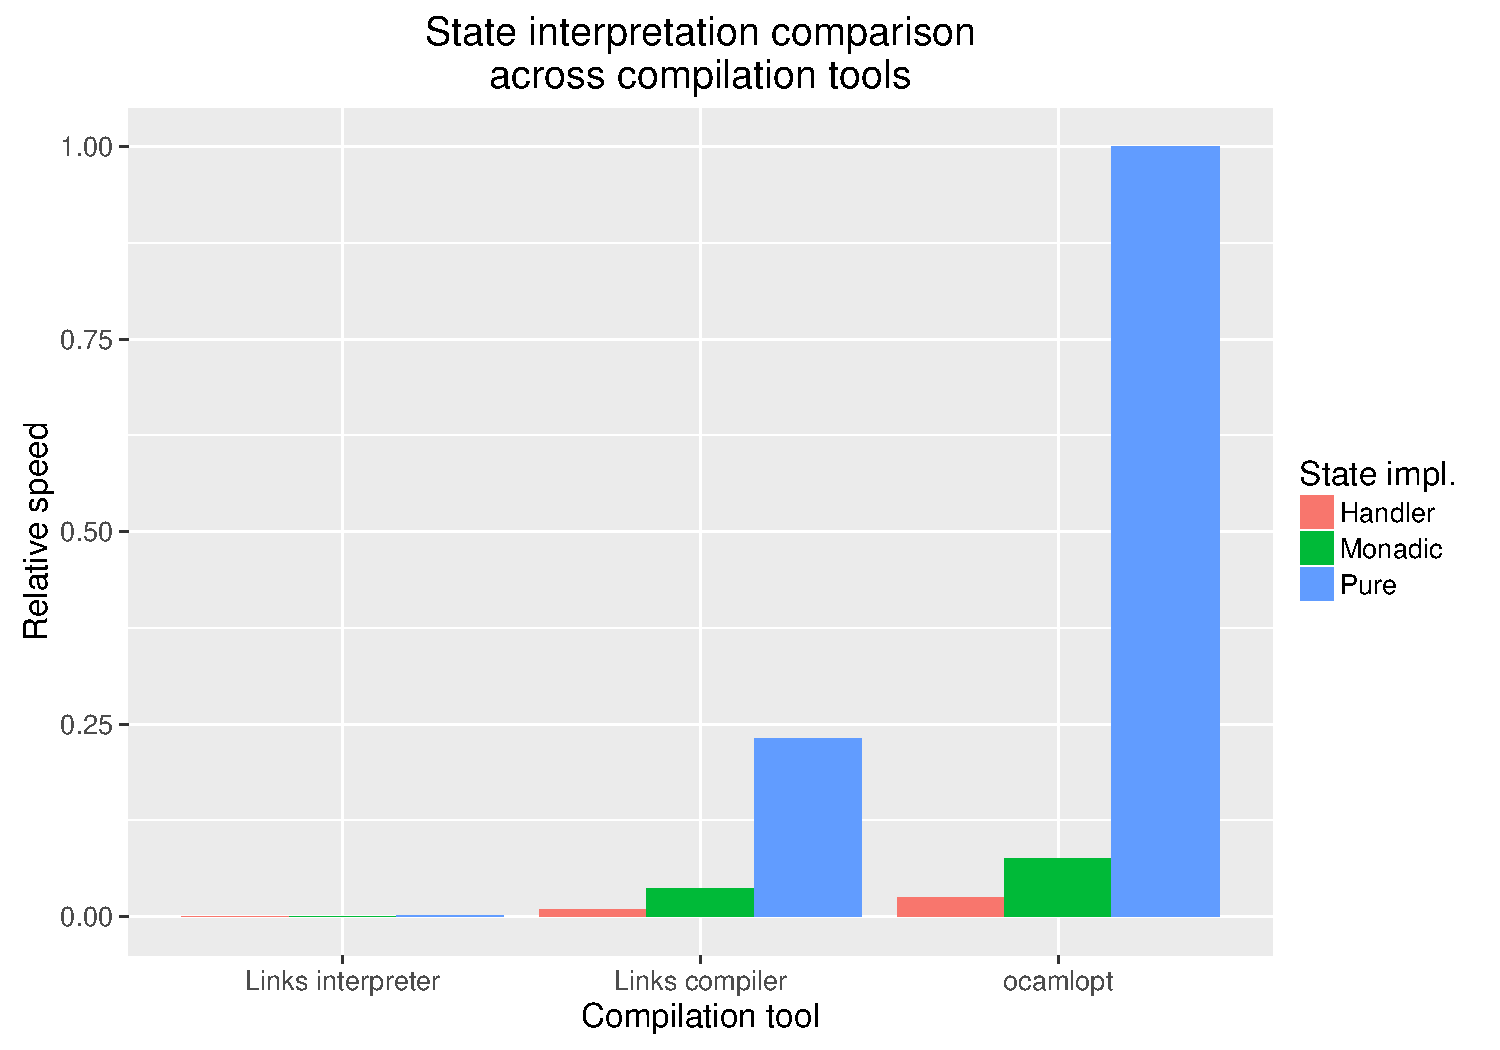
\includegraphics[scale=0.6]{plots/stateAll.pdf}
\caption{Bar plot of data from Table~\ref{tbl:state-all} (higher is
  better).}\label{fig:state-all}
\end{figure}

% \begin{table}
% \centering
% \begin{tabular}{|l | r | r | r |}
% \hline
% Compilation tool & ocamlopt & Links interpreter & Links compiler \\
% \hline
% Relative speed   & *0.0     & 0.0               & 0.0\\
% \hline
% \end{tabular}
% \caption{State handler comparison. * is baseline.}\label{fig:state-handler-all}
% \end{table}

\subsection{Recovering performance}
\label{sec:state-recover}

We noted that the state programs compiled using the Links compiler
performed rather poorly compared to the baseline implementation in
OCaml. In this section we will try to account for difference in
performance. Moreover, we will demonstrate how we can equilibrise some
of the performance.

Given that the Links compiler conservatively implements the state
handler as a multi-shot handler we can try to enforce linearisation of
handlers in order to obtain some insight into how expensive it is to
copy the continuation.

However, linearisation does not explain the poor performance of the
pure state program. The explanation is, again, that the Links compiler
does not perform any optimisations. In particular, the polymorphic
built-in comparison operators are translated into their generic
counterparts in OCaml/Lambda. This means that the equality operator in
the state program gets translated into the generic equality operator
in OCaml instead of the more efficient, hardware supported integer
comparison operator. Since the equality testing occurs 10000000 times
in the state program the overhead in occurred by the generic operator
is going to be significant. This claim is supported by the results
shown in Table~\ref{tbl:state-all-recovered}. The ``Links
compiler/lin+eq'' denotes a special version of the Links compiler in
which we have hand-coded handlers linearisation and equality testing
specialisation.

%                   names      Handler      Monadic        Pure
% 1        Links compiler 0.0089798851 0.0369276219 0.231481481
% 2     Links interpreter 0.0002951489 0.0001298283 0.001687479
% 3              ocamlopt 0.0247770069 0.0753012048 1.000000000
% 4 Links compiler/lin+eq 0.0222024867 0.0437828371 1.190476190
\begin{table}
\centering
\begin{tabular}{| l || r | r | r |}
\cline{2-4}
\multicolumn{1}{c|}{~} & \multicolumn{3}{c|}{\textbf{State implementation}} \\
\cline{1-4}
\multicolumn{1}{|l||}{\textbf{Compilation tool}}  & Handler & Monadic & Pure \\
\hline
  Links interpreter & 0.0030   & 0.0001  & 0.0017 \\
\hline
  Links compiler    & 0.0089   & 0.0370 & 0.2315 \\
\hline
  ocamlopt          & 0.0250   & 0.0753  & *1.0000 \\
\hline
  Links compiler/lin+eq & 0.0222 & 0.0438 & 1.1905 \\
\hline
\end{tabular}
\caption{Comparison of state implementations. The component marked
  with * is the baseline.}\label{tbl:state-all-recovered}
\end{table}
\begin{figure}
\centering
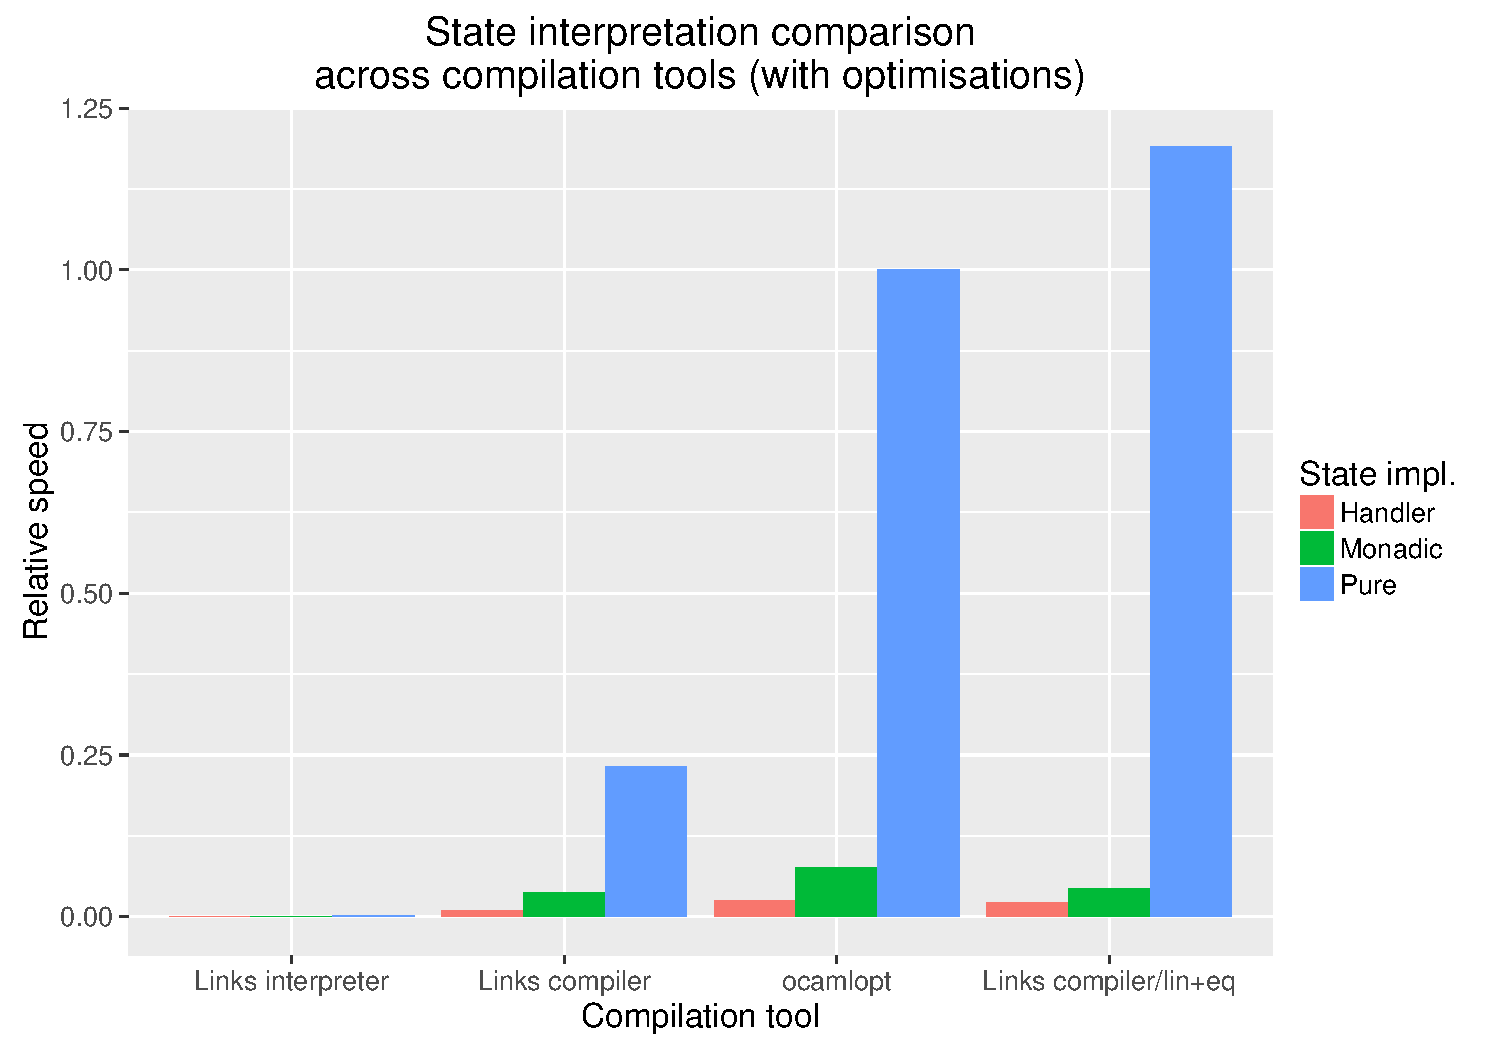
\includegraphics[scale=0.6]{plots/stateAll_recovered.pdf}
\caption{Bar plot of data in Table~\ref{tbl:state-all-recovered} (higher is better).}\label{fig:state-all-recovered}
\end{figure}

Figure~\ref{fig:state-all-recovered} visualises the data. We achieve
significant speed ups. In particular, the Links compiler out performs
the OCaml compiler on the pure state program. The Links compiler
achieves roughly 19\% performance than the OCaml compiler on that
particular program. The explanation for this difference is rather
subtle: it relates to the module system of OCaml and the lack of a
module system in Links. Every OCaml source file constitutes a
module. Furthermore, an accessible top-level function in one module
can be invoked from another module in OCaml. In order to support
cross-module invocation of functions OCaml maintains per module a
global table which contains the callable top-level functions of that
particular module. Since the function \lstinline$count$ in the state
program is a global function it gets registered in the global table,
which means the first invocation of \lstinline$count$ costs one look
up in the global table in order to locate the function. In Links every
function is resolved statically, because there is no concept of cross
module function invocation. Therefore, we do not pay the initial look
up cost.

Unsurprisingly, linearisation speeds up the handler significantly. It
almost brings it on par with the OCaml
implementation. Figure~\ref{fig:statehandler-all} depicts a comparison
of the different state handler implementations relative to the OCaml
implementation. The figure includes an additional special version of
the Links compiler (denoted ``Links compiler/lin'') which only
performs linearisation of handlers. We see that linearisation accounts
for a large chunk of the overall improvement. Even with both
optimisations the performance is still about 12\% worse than the OCaml
implementation. It is likely that we can close this gap by fine tuning
the compiler.

\begin{figure}[H]
\centering
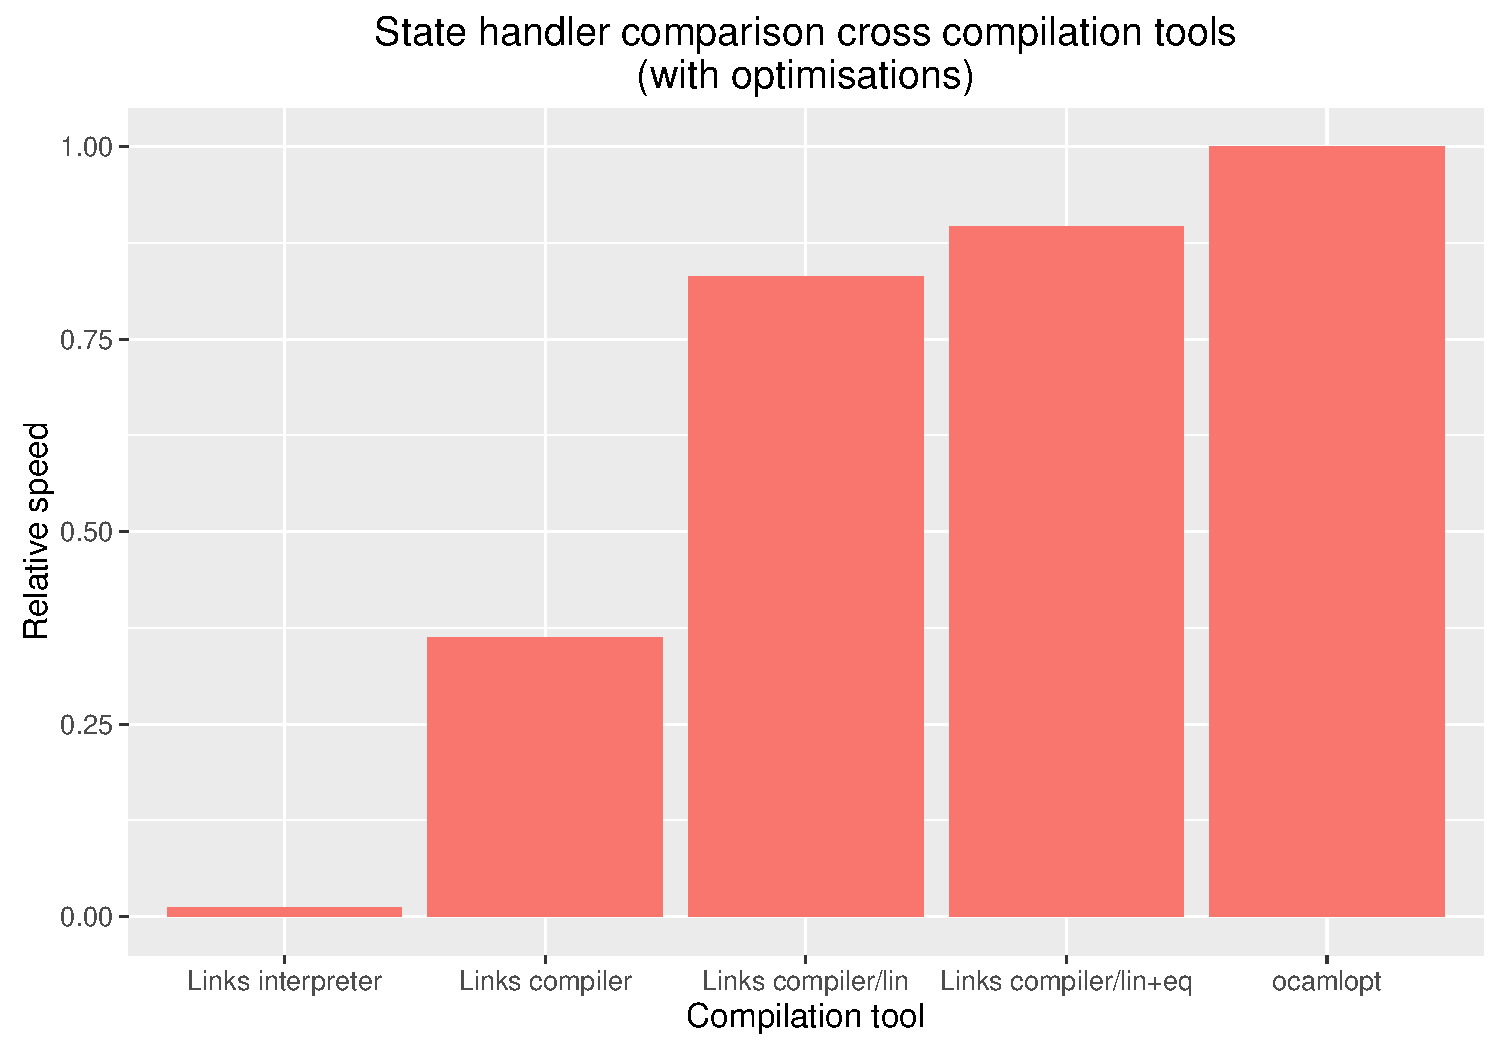
\includegraphics[scale=0.6]{plots/statehandlerAll.pdf}
\caption{Plot of handler data from Table~\ref{tbl:state-all-recovered}
  with the addition of ``Compiler/lin'' (higher is
  better).}\label{fig:statehandler-all}
\end{figure}

\section{Queens benchmark}
\label{sec:queens-eval}

\begin{table}[H]
\centering
\begin{tabular}{| l | r | r | r | r |}
\hline
N  & 8 & 12 & 16 & 20 \\
\hline
  Links interpreter (ms) & 0.0 & 0.0 & 0.0 & 0.0\\
\hline
  Links compiler    (ms) & 0.0 & 0.0 & 0.0 & 0.0\\
\hline
\end{tabular}
\caption{$N$-queens benchmark.}\label{tbl:queens}
\end{table}

\section{Concurrency implementation}
\label{sec:concur-label}

We encoded the concurrency model of Links using handlers in
Chapter~\ref{ch:concurrency}. The motivation was to replace the
built-in implementation. It is interesting to compare the handler
encoding against the built-in implementation. Table~\ref{tbl:sieve}
contains the data obtained by running the Sieve example
(c.f. Sections~\ref{sec:sieve-example} and
\ref{sec:links-model-handlers-example}) with different parameters. 
%   SieveN Compiler Builtin Interpreter
% 1     27       21      56         992
% 2     47       38      65        2473
% 3     80      103      95        9589
% 4    111      231     136       24301
% 5    140      409     186       48679
% 6    169      658     247       84822
\begin{table}[H]
\centering
\begin{tabular}{| l | r | r | r | r | r | r |}
\hline
N  & 101 & 201 & 401 & 601 & 801 & 1001\\
\hline
Number of process & 27 & 47 & 80 & 111 & 140 & 169\\
\hline
\hline
  Interpreter/handlers (ms) & 992  & 2473 & 9589 & 24301  & 48679  & 84822\\
\hline
  Interpreter/built-in (ms) & 56 & 65 & 95 & 136 & 186 & 247\\
\hline
  Compiler    (ms) & 21 & 38 & 103 & 231  & 409  & 658\\
\hline
\end{tabular}
\caption{Concurrency implementation scaling (lower is better).}\label{tbl:sieve}
\end{table}
The variable $N$ is the upper bound given to the generator process,
the second row lists the number of concurrent processes that were
spawned. Figure~\ref{fig:sieve-plot} displays a line plot of the
data. As we might expect the interpreter with the handler
implementation performs poorly compared to the built-in and the
compiler
implementations. Figure~\ref{fig:sieve-handler-interpreter-plot} zooms
in on the two implementations. We see that compiler implementation
does not scale as well as the built-in implementation. When we have
about 80 processes running the compiler implementation starts
performing worse than the other.

The interpreter appears to scale surprisingly well. Needless to say,
our compiled concurrency implementation should not really be
out-performed by an interpreted version. If we enable the
optimisations from Section~\ref{sec:state-recover} then we see that
the compiled implementation performs better than the
interpreter. Table~\ref{tbl:sieve-recovered} shows the data, and
Figure~\ref{fig:sieve-recovered-plot} displays a visualisation of the
data. In particular, it appears that the compiled implementation
scales as nicely as the built-in implementation.

\begin{figure}[H]
\centering
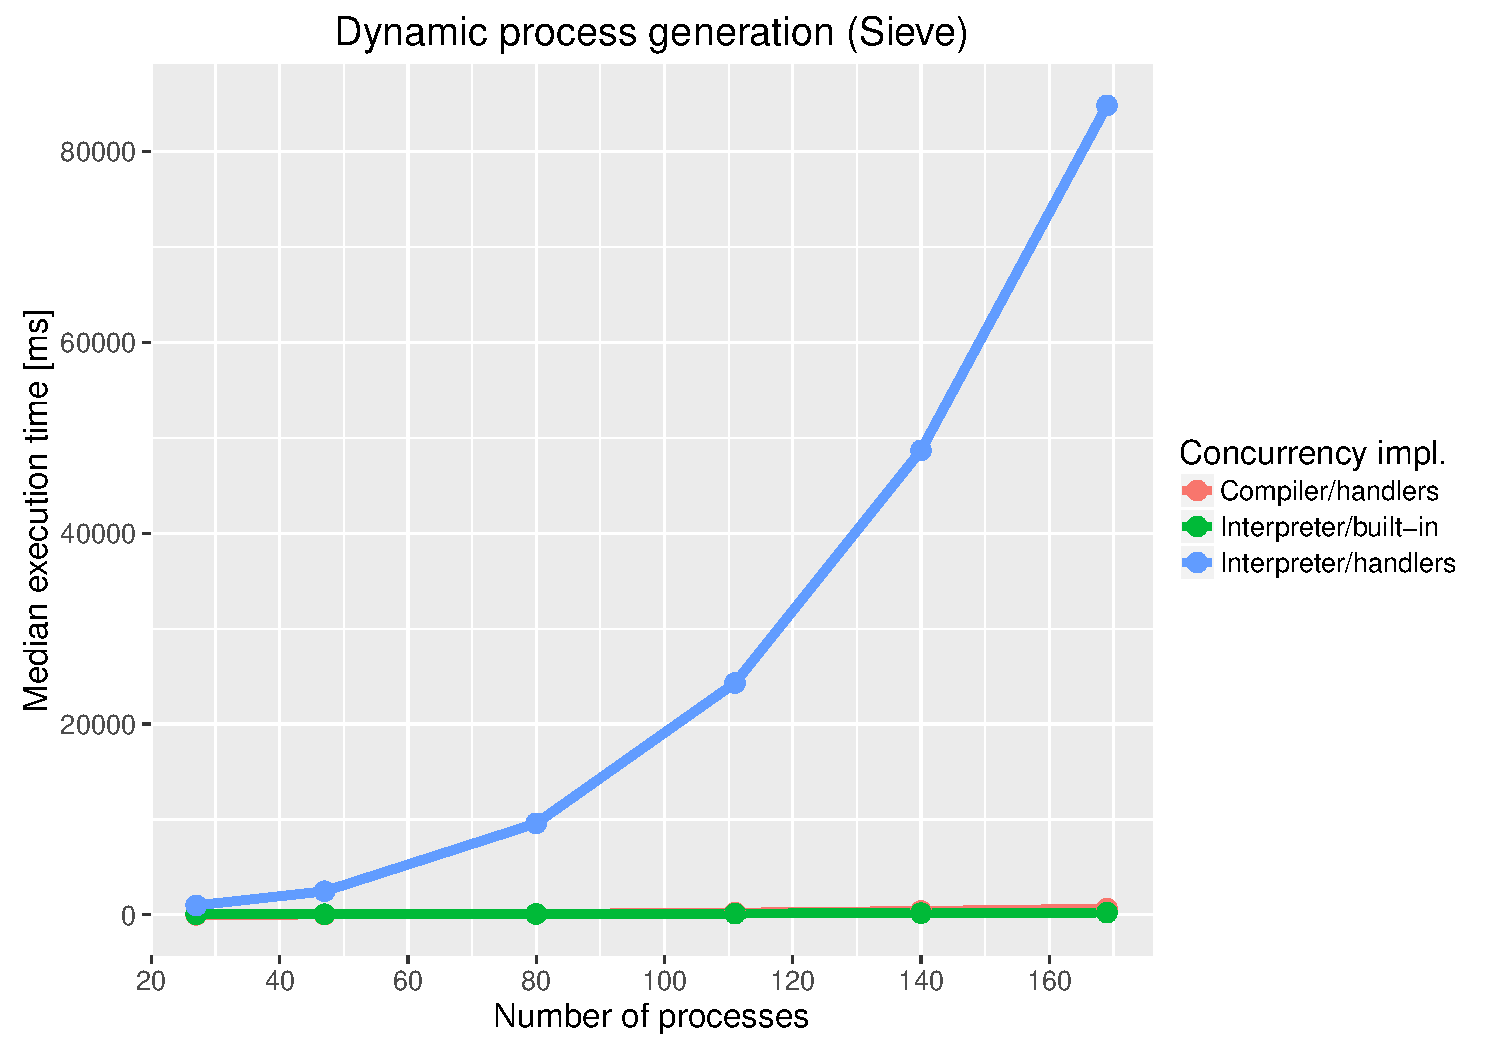
\includegraphics[scale=0.55]{plots/sieve.pdf}
\caption{Concurrency implementation scaling (lower is better).}\label{fig:sieve-plot}
\end{figure}

\begin{figure}
\centering
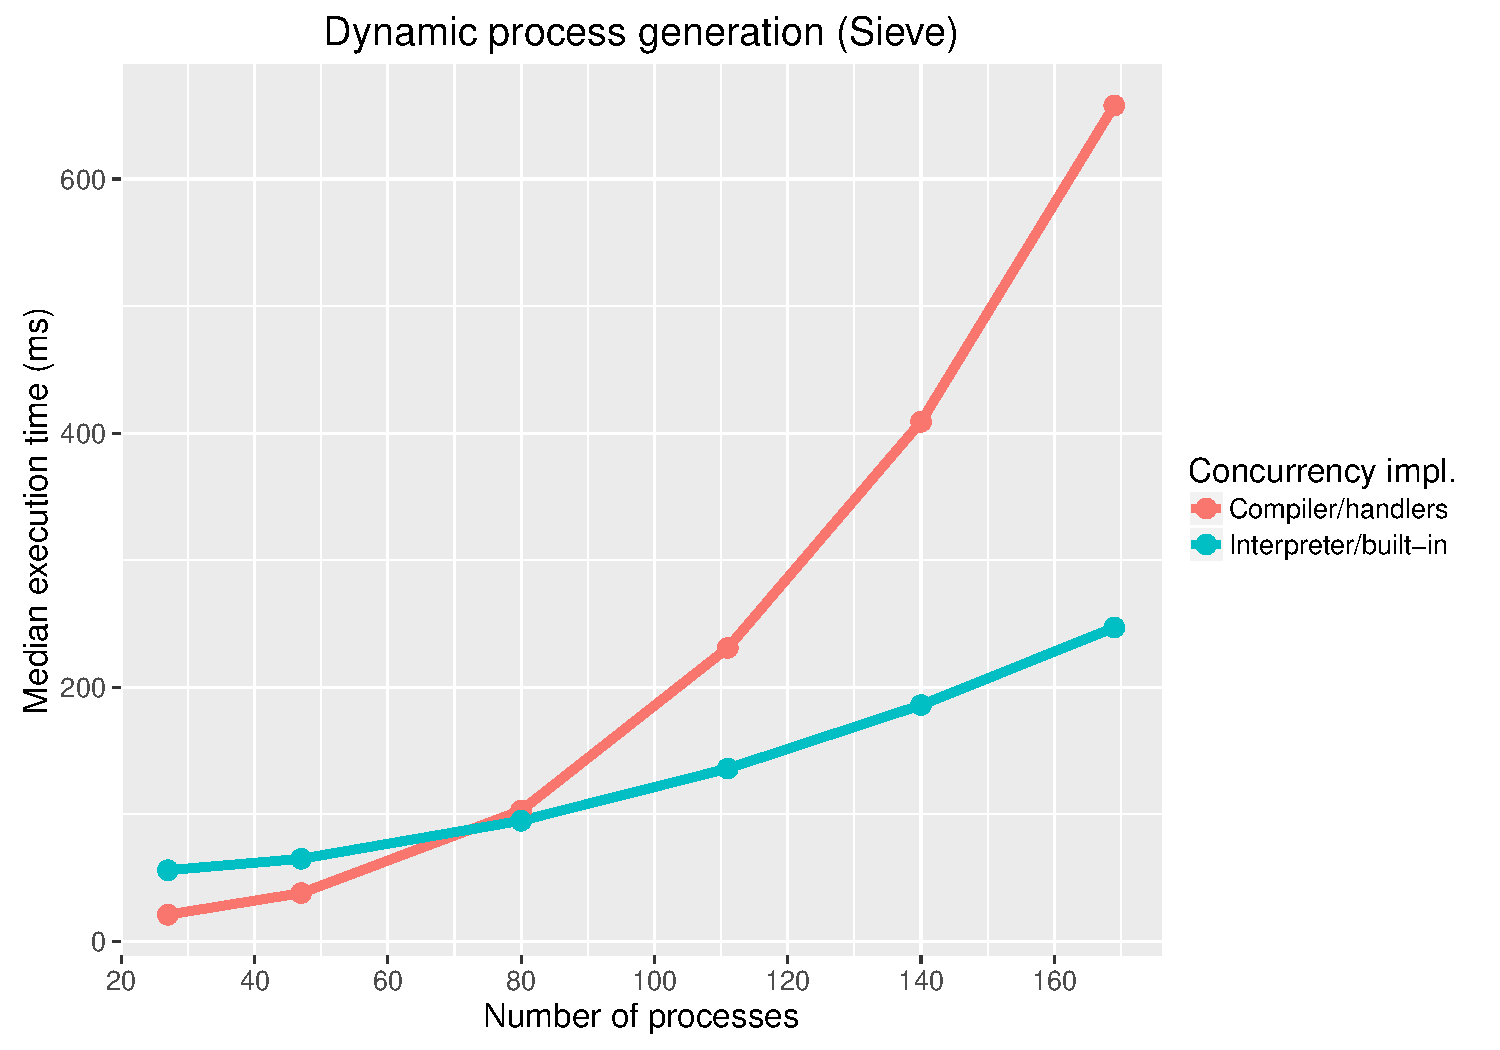
\includegraphics[scale=0.55]{plots/sieve_compiler-interpreter.pdf}
\caption{Compiler/handler vs Interpreter/built-in (lower is better).}\label{fig:sieve-handler-interpreter-plot}
\end{figure}


%   SieveN Compiler Builtin CompilerOpt
% 1     27       21      56          17
% 2     47       38      65          22
% 3     80      103      95          36
% 4    111      231     136          61
% 5    140      409     186          99
% 6    169      658     247         153
\begin{table}[H]
\centering
\begin{tabular}{| l | r | r | r | r | r | r | r |}
\hline
N  & 101 & 201 & 401 & 601 & 801 & 1001 \\
\hline
Number of process & 27 & 47 & 80 & 111 & 140 & 169 \\
\hline
\hline
  Interpreter/built-in (ms) & 56 & 65 & 95 & 136 & 186 & 247 \\
\hline
  Compiler    (ms) & 21 & 38 & 103 & 231  & 409  & 658  \\
\hline 
  Compiler/lin+eq (ms) & 17 & 22 & 36 & 61 & 99 & 153 \\
\hline
\end{tabular}
\caption{Concurrency implementation scaling with hand-coded optimisations.}\label{tbl:sieve-recovered}
\end{table}

\begin{figure}[H]
\centering
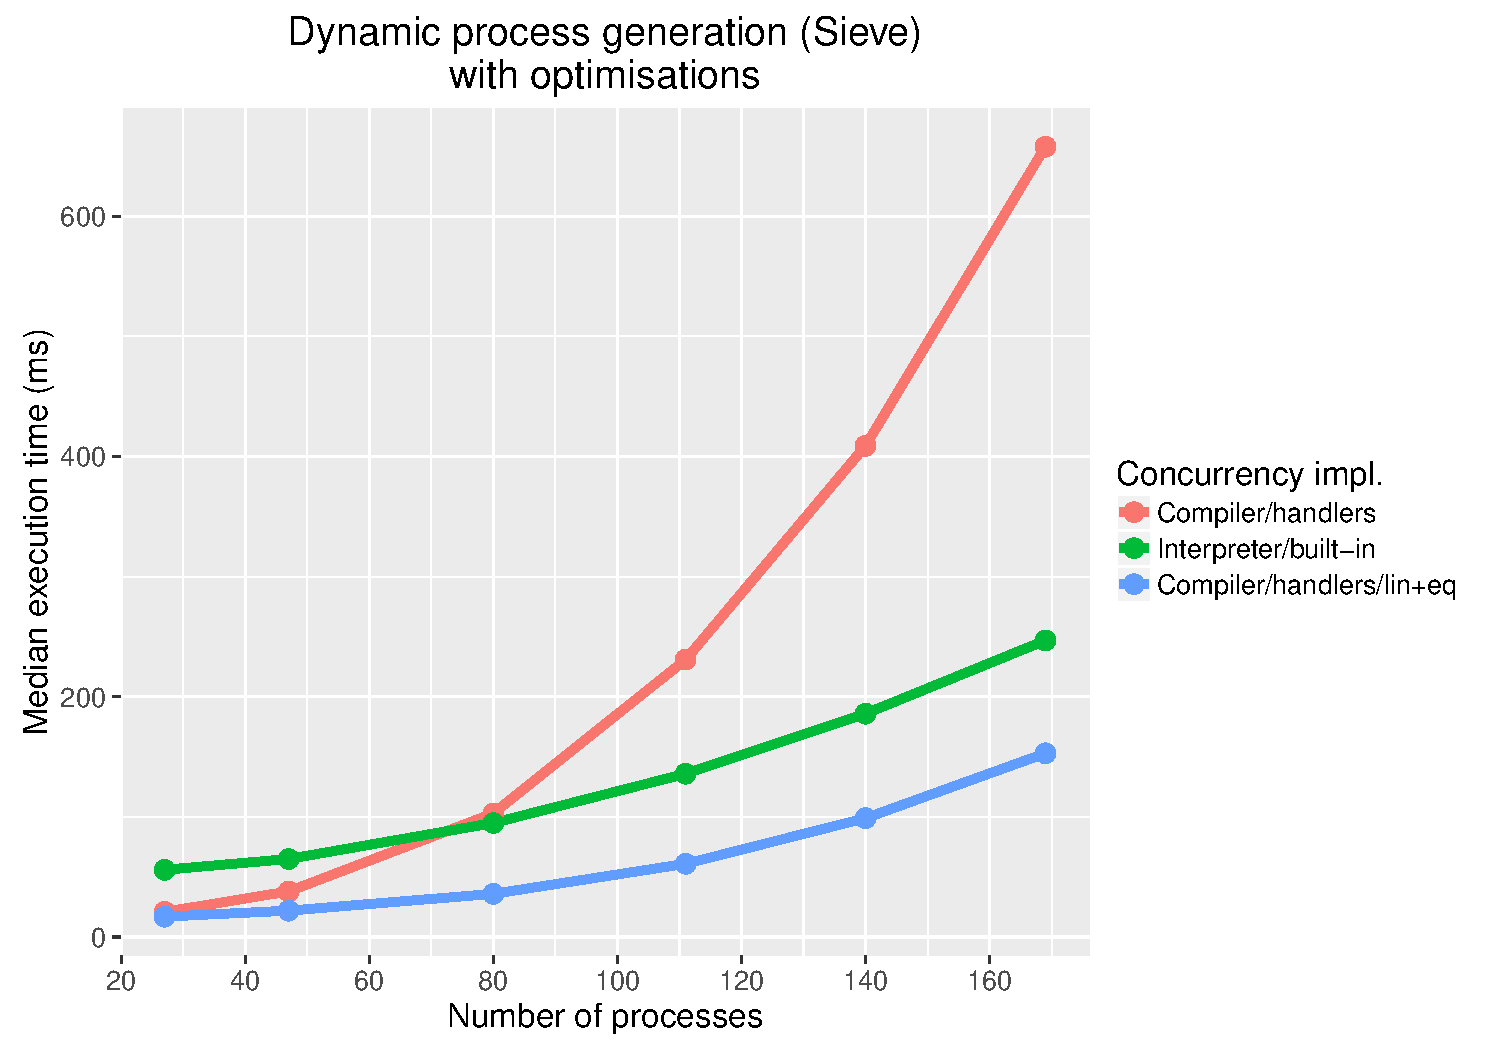
\includegraphics[scale=0.55]{plots/sieve_recovered.pdf}
\caption{Line plot of data from Table~\ref{tbl:sieve-recovered}.}\label{fig:sieve-recovered-plot}
\end{figure}

%%
%% Formalisation
%%
% \chapter{A calculus of handlers and rows}
% \label{sec:lambe-eff-row}

% In this section, we present a type and effect system and a small-step
% operational semantics for \Calc (pronounced ``lambda-eff-row''), a
% Church-style row-polymorphic call-by-value calculus for effect
% handlers.
% %
% This core calculus captures the essence of the Links IR.
% %
% We prove that the operational semantics is sound with respect to the
% type and effect system.

% A key advantage of row polymorphism is that it integrates rather
% smoothly with Hindley-Milner type inference. We concern ourselves only
% with the explicitly-typed core language, as the treatment of type
% inference is quite standard.

% The design of \Calc is inspired by the $\lambda$-calculi of
% \citet{Kammar2013}, \citet{Pretnar2015}, and \citet{Lindley2012}.
% %
% As in the work of \citet{Kammar2013}, each handler can have its own
% effect signature. As in the work of \citet{Pretnar2015}, the
% underlying formalism is fine-grain call-by-value~\cite{LevyPT03},
% which names each intermediate computation like in A-normal
% form~\cite{Flanagan1993}, but unlike A-normal form is closed under
% $\beta$-reduction. As in the work of \citet{Lindley2012}, the effect
% system is based on row polymorphism.

% \section{Types}
% The grammars of types, effects, kinds, and type and kind environments
% are given in Figure~\ref{fig:types-syntax}.

% \begin{figure}
% Types
% \begin{syntax}
% \slab{Value types}    &A,B  &::= & %\Bool \mid \Int
%                                       A \to C
%                                \mid  \forall \alpha^K.C \\
%                              &&\mid& \Record{R} \mid [R]
%                                \mid  C \Rightarrow D \mid \alpha \\
%                                %% \mid  \Harrow{A}{E}{B}{E'} \mid \alpha \\
% \slab{Computation types} 
%                       &C,D  &::= & A \eff E \\
% \slab{Effect types}   &E    &::= & \{R\}\\
% \slab{Row types}      &R    &::= & \ell : P;R \mid \rho \mid \cdot \\
% \slab{Presence types} &P    &::= & \Pre{A} \mid \Abs \mid \theta\\
% %\slab{Labels}         &\ell &    &                \\
% \slab{Kinds}          &K    &::= & \Type \mid \Row_\mathcal{L} \mid \Presence\\
% \slab{Label sets}     &\mathcal{L} &::=& \emptyset \mid \{\ell\} \uplus \mathcal{L}\\
% %\slab{Type variables} &\alpha, \rho, \theta& \\
% \slab{Type environments} &\Gamma &::=& \cdot \mid \Gamma, x:A \\
% \slab{Kind environments} &\Delta &::=& \cdot \mid \Delta, \alpha:K \\
% \end{syntax}
% \caption{Types, effects, kinds, and environments}
% \label{fig:types-syntax}
% \end{figure}

% \paragraph{Value Types}
% %The base types are integers and booleans.
% The function type $A \to C$ takes an argument of type $A$ and returns
% a computation of type $C$.
% %% The effect signature enumerates the
% %% operations that the function may perform during evaluation.
% The polymorphic type $\forall \alpha^K .\, C$ is parameterised by a
% type variable $\alpha$ of kind $K$. The record type $\Record{R}$
% represents records with fields given by labels of row $R$. Dually, the
% variant type $[R]$ represents a sum of fields tagged by the labels of
% row $R$. The handler type $C \Rightarrow D$ transforms a computation
% of type $C$ into a computation of type $D$.

% \paragraph{Computation Types}
% A computation type $A \eff E$ is given by a value type $A$ and an
% effect $E$, which specifies the operations that the computation may
% perform.

% \paragraph{Row Types}
% Effect types, records and variants are defined in terms of rows.
% A row type embodies a collection of distinct labels, each of which is
% annotated with a presence type. A presence type indicates whether a
% label is \emph{present} with some type $A$ ($\Pre{A}$), \emph{absent}
% ($\Abs$) or \emph{polymorphic} in its presence ($\theta$).

% Row types are either \emph{closed} or \emph{open}. A closed row type
% ends in~$\cdot$, whilst an open row type ends with a \emph{row
%   variable} $\rho$. Furthermore, a closed row term can have only the
% labels explicitly mentioned in its type. Conversely, the row variable
% in an open row can be instantiated with additional labels. We identify
% rows up to reordering of labels, for instance, we consider the
% following two rows equivalent:
% \[ \ell_1 : P_1; \cdots; \ell_n : P_n \equiv \ell_n : P_n; \cdots ; \ell_1 : P_1. \]
% The unit and empty type are definable in terms of row types. We define
% the unit type as the empty, closed record, that is,
% $\Record{\cdot}$. Similarly, we define the empty type as the empty,
% closed variant $[\cdot]$. Usually, we usually omit the $\cdot$ for
% closed rows.

% \paragraph{Kinds}
% We have three kinds: $Type$, $\emph{Row}_\mathcal{L}$ and $Presence$
% which classify value types, row types and presence types,
% respectively. Row kinds are annotated with a set of labels
% $\mathcal{L}$. The kind of a complete row is
% $Row_{\mathcal{\emptyset}}$. More generally, the kind
% $Row_{\mathcal{L}}$ denotes a partial row which cannot mention the
% labels in $\mathcal{L}$.
% %

% \paragraph{Type Variables}
% We let $\alpha$, $\rho$ and $\theta$ range over type variables. By
% convention we use $\alpha$ for value type variables or for type
% variables of unspecified kind, $\rho$ for type variables of row kind,
% and $\theta$ for type variables of presence kind.

% \paragraph{Type and Kind Environments}
% Type environments map term variables to their types and kind
% environments map type variables to their kinds.

% \section{Terms}
% \begin{figure}
% \begin{syntax}
%                              % SL: no need for constants in the core calculus
% %\slab{Constants}     &c    &::= & n \mid \True \mid \False \\
% \slab{Values}        &V,W  &::= & x
%                              %\mid c
%                              \mid \lambda x^A .\, M \mid \Lambda \alpha^K .\, M  \\
%                      &     &\mid& \Record{} \mid \Record{\ell = V;W} \mid (\ell\, V)^R \\
%                      &     &    &\\
% \slab{Computations}  &M,N  &::= & V\,W \mid V\,A\\
%                      &     &\mid& \Let\; \Record{\ell=x;y} \revto V \; \In \; N\\
%                      &     &\mid& \Case\; V \{\ell\; x \mapsto M; y \mapsto N\} \mid \Absurd^C V\\
%                      &     &\mid& \Return\; V \\
%                      &     &\mid& \Let \; x \revto M \; \In \; N\\
%                      &     &\mid& (\Do \; \ell \; V)^E \\
%                      &     &\mid& \Handle \; M \; \With \; H\\
%                      &     &    &\\
% \slab{Handlers}      &H    &::= & \{ \Return \; x \mapsto M \} \\
%                      &     &\mid& \{ \ell \; x \; k \mapsto M \} \uplus H \\
% %% \slab{Integers}      &n    &      \\
% %% \slab{Variables}     &x,y,z,k &    & \\
% \end{syntax}

% \caption{Term Syntax}
% \label{fig:term-syntax}
% \end{figure}
% The terms are given in Figure~\ref{fig:term-syntax}. We let $x,y,z,k$
% range over term variables. By convention, we use $k$ to denote
% continuation names. %We let $n$ range over integer constants.

% The syntax partitions terms into values, computations and
% handlers. 
% %
% Value terms comprise variables ($x$), %constants ($c$),
% lambda abstraction ($\lambda x^A . \, M$), type abstraction ($\Lambda
% \alpha^K . \, M$), and the introduction forms for records and
% variants. Records are introduced using the empty record $\Record{}$
% and record extension $\Record{\ell = V; W}$, whilst variants are
% introduced using injection $(\ell\, V)^R$ which injects a field with
% label $\ell$ and value $V$ into a row whose type is $R$. We include
% the row type annotation in order to support bottom-up type
% reconstruction.

% All elimination forms are computation terms. Abstraction and type
% abstraction are eliminated using application ($V\,W$) and type
% application ($V\,A$) respectively.
% %
% The record eliminator $(\Let \; \Record{\ell=x;y} \revto V \; \In \;
% N)$ splits a record $V$ into $x$, the value associated with $\ell$,
% and $y$, the rest of the record. Non-empty variants are eliminated
% using the case construct ($\Case\; V\; \{\ell\; x \mapsto M; y \mapsto
% N\}$), which evaluates the computation $M$ if the tag of $V$ matches
% $\ell$, otherwise it falls through to $y$ and evaluates $N$.  The
% elimination form for empty variants is ($\Absurd^C V$). A trivial
% computation $(\Return\;V)$ returns value $V$. The expression $(\Let \;
% x \revto M \; \In \; N)$ evaluates $M$ and binds the result value to
% $x$ in $N$.

% The construct $(\Do \; \ell \; V)^E$ invokes an operation $\ell$ with
% value argument $V$. The handle construct $(\Handle \; M \; \With \;
% H)$ runs a computation $M$ with handler definition $H$. A handler
% definition $H$ consists of a return clause $\Return \; x \mapsto M$
% and a possibly empty set of operation clauses $\{\ell_i \; x_i \; k_i
% \mapsto M_i\}_i$. The return clause defines how to handle the final
% return value of the handled computation, which is bound to $x$ in $M$.
% %
% The $i$-th operation clause binds the operation parameter to $x_i$ and
% a the continuation $k_i$ in $M_i$.

% We write $Id(M)$ for $\Handle \;M\; \With \; \{\Return\;x \mapsto
% x\}$.
% %
% We write $H(\Return)$ for the return clause of $H$ and $H(\ell)$ for
% the set of either zero or one operation clauses in $H$ that handle the
% operation $\ell$. We write $dom(H)$ for the set of operations handled
% by $H$.
% %
% As our calculus is Church-style, we annotate various term forms with
% type or kind information (term abstraction, type abstraction,
% injection, operations, and empty cases); we sometimes omit these
% annotations.

% %% SL: possibly a bit draconian, but I think we can do without the
% %% detail here.

% %% The terms of \Calc are written in a style reminiscent of
% %% \emph{A-normal form} (ANF). ANF is a direct style intermediate
% %% language in which every intermediate computation is let-bound
% %% \cite{Flanagan1993}. As a consequence application consist of a value
% %% applied to another value. For example, consider the Links expression
% %% \lstinline$f(g(42))$, we must let bind the argument of \lstinline$f$
% %% in order to bring the expression into ANF; we do not need to let bind
% %% the argument of \lstinline$g$, since it is already a value, thus we
% %% obtain the following ANF expression:
% %% \[
% %% \Let\; x \revto g\,42\; \In \; f\, x.
% %% \]
% %% However, ANF is not closed under $\beta$-reduction
% %% \cite{Sabry1996,Kennedy2007}, since function application can lead to
% %% nested \Let{}s. Consider the following example, which is adapted from
% %% \citet{Sabry1996}:
% %% \[ 
% %%   \Let\; x \revto (\lambda y . \, \Let\; z \revto f \, a \;\In \; M) \, b \; \In\; N
% %% \]
% %% which $\beta$-reduces to 
% %% \[
% %%   \Let\; x \revto (\Let\; z \revto f \, a \;\In \; M) \; \In\; N
% %% \]
% %% which is not in ANF, because $x$ is bound to a computation rather than
% %% a value. ANF can be recovered by adding a normalisation step
% %% \cite{Sabry1996}.  We simplify our presentation by permitting nested
% %% let-bindings and handlers to be applied directly to computations. The
% %% resulting calculus is closer to fine-grained
% %% call-by-value~\cite{LevyPT03}.

% %% ,
% %% therefore we say that \Calc-terms are in \emph{relaxed A-normal
% %%   form} (RANF).

% % As an example consider the translation of the Links expression \linksify{f(g(42),\{ var y = 1; h(y) \})} into its ANF. For clarity, we highlight the reducible term with a box:
% % \begin{align*}
% %             &  \fbox{\linksify{f(g(42),\{ var y = true; h(y) \})}}\\
% % \Rightarrow &\quad\Let \; x_1 \revto g \; 42 \; \In\\
% %             &\quad\quad\fbox{\linksify{f($x_1$,\{ var y = true; h(y) \})}}\\
% % \Rightarrow &\quad\Let \; x_1 \revto g \; 42 \; \In\\
% %             &\quad\quad\Let \; y \revto \Return \; \True \; \In\\
% %             &\quad\quad\quad\fbox{\linksify{f($x_1$,h($y$))}}\\
% % \Rightarrow &\quad\Let \; x_1 \revto g \; 42 \; \In\\
% %             &\quad\quad\Let \; y \revto \Return \; \True \; \In\\
% %             &\quad\quad\quad\Let \; x_2 \revto h \; y \; \In\\
% %             &\quad\quad\quad\quad(f \; x_1)\; x_2
% % \end{align*}
% % Accordingly, the function \linksify{f} is applied only to value terms. Every subexpression gets decomposed into a single value gradually. As a consequence every subexpression has been explicitly named, thus in this respect, ANF is similar to the predominant imperative Static Single Assignment form.

% \section{Static Semantics}
% \label{sec:typing}
% The kinding rules are given in Figure~\ref{fig:kinding} and the typing
% rules are given in Figure~\ref{fig:typing}.

% The kinding judgement $\Delta \vdash \alpha : K$ asserts that the type
% variable $\alpha$ has kind $K$ in kind environment $\Delta$. The value
% typing judgement $\typv{\Delta;\Gamma}{V : A}$ states that value term
% $V$ has type $A$ under kind environment $\Delta$ and type environment
% $\Gamma$. The computation typing judgement $\typc{\Delta;\Gamma}{M :
%   A}{E}$ states that the term $M$ has type $A$ and effects $E$ under
% kind environment $\Delta$ and type environment $\Gamma$. In typing
% judgements, we implicitly assume that $\Gamma$, $E$ and $A$ are
% well-kinded with respect to $\Delta$. We define the functions
% $FTV(\Gamma)$ and $FTV(E)$ to be the set of free type variables in
% $\Gamma$ and $E$, respectively.
% %
% %% We write $FTV(\Gamma,E)$ as shorthand for $FTV(\Gamma) \cup FTV(E)$.

% The kind and typing rules are mostly straightforward. The interesting
% typing rules are \tylab{Handle} and the two handler rules. The
% \tylab{Handle} rule states that $\Handle\; M\; \With\; H$ produces a
% computation of type $B$ given that the computation $M$ is typeable
% under effect context $E$, and that $H$ is a handler which transforms a
% computation of type $A$ with effect signature $E$ into another
% computation of type $B$ with effect signature $E'$.

% The \tylab{Handler} rule is crucial. The input effect $E$ and the
% output effect $E'$ must share the same suffix $R$. This means that
% $E'$ must explicitly mention each of the operations $\ell_i$, whether
% that be to say that an $\ell_i$ is present with a given type
% signature, absent, or polymorphic in its presence. The row $R$
% describes the operations that are forwarded. It may include a
% row-variable, in which case an arbitrary number of effects may be
% forwarded by the handler.
% %
% The typing of the return clause is straightforward. In the typing of
% each operation clause, the continuation returns the output computation
% type $D$. Thus, we are here defining \emph{deep}
% handlers~\cite{Kammar2013} in which the handler is implicitly wrapped
% around the continuation, such that any subsequent operations are
% handled uniformly by the same handler.
% %
% The Links implementation also supports \emph{shallow}
% handlers~\cite{Kammar2013}, in which the continuation is instead
% annotated with the input effect and one has to explicitly reinvoke the
% handler after applying the continuation inside an operation clause.

% %% \todo{Insert a forward reference to discussion of shallow handlers
% %%   elsewhere.}

% %% The \tylab{Deep} and \tylab{Shallow} rules for handlers describe how
% %% to type deep and shallow handlers, respectively. The two rules are
% %% similar, but differ crucially in their typing of the continuation
% %% parameter $k$. The different typing is due to their different
% %% behaviour. A deep handler wraps itself around continuations such that
% %% any subsequent operations are handled uniformly. Therefore the return
% %% type of a continuation type must match the input type of the
% %% \Return{} case, and in particular, its effect signature must be the
% %% same as the handler's output effect signature $E'$. Conversely, in a
% %% shallow handler the continuation is annotated with the input effect
% %% signature $E$ rather than the output effect signature. Moreover, the
% %% return type $A$ is the same as return type of the handled
% %% computation. Shallow handlers do not wrap themselves around the
% %% continuation, therefore the continuation must be applied explicitly to
% %% handler which has to handle the next operation
% %% invocation. Consequently, operations may be handled non-uniformly.

% %% For both handler types the input effect signature is a disjoint union
% %% of operation signatures, that the handler directly interprets, and
% %% some set $E_f$. The metavariable $E_f$ can be instantiated with a row
% %% variable to include operations that are not explicitly mentioned by
% %% the handler.

% \begin{figure}
% \begin{mathpar}
% % alpha : K
%   \inferrule*[Lab=\klab{TyVar}]
%     { }
%     {\Delta, \alpha : K \vdash \alpha : K}

% % forall alpha : K . A : Type
%   \inferrule*[Lab=\klab{Forall}]
%     { \Delta, \alpha : K \vdash A : \Type \\
%       \Delta, \alpha : K \vdash R : \Row_\emptyset}
%     {\Delta \vdash (\forall \alpha^K . \, A \eff \{R\}) : \Type}
% %%
% %% % Int : Type
% %%   \inferrule*[Lab=\klab{Int}]
% %%     { }
% %%     {\Delta \vdash \Int : \Type}
% %%
% %% % Bool : Type
% %%   \inferrule*[Lab=\klab{Bool}]
% %%     { }
% %%     {\Delta \vdash \Bool : \Type}

% % A -E-> B, A : Type, E : Row, B : Type
%   \inferrule*[Lab=\klab{Fun}]
%     { \Delta \vdash A : \Type \\
%       \Delta \vdash R : \Row_\emptyset  \\
%       \Delta \vdash B : \Type
%     }
%     {\Delta \vdash (A \to B \eff \{R\}) : \Type}

% % Record
%   \inferrule*[Lab=\klab{Record}]
%     { \Delta \vdash R : \Row_\emptyset}
%     {\Delta \vdash \Record{R} : \Type}

% % Variant
%   \inferrule*[Lab=\klab{Variant}]
%     { \Delta \vdash R : \Row_\emptyset}
%     {\Delta \vdash [R] : \Type}

% % Present
%   \inferrule*[Lab=\klab{Present}]
%     {\Delta \vdash A : \Type}
%     {\Delta \vdash \Pre{A} : \Presence}

% % Absent
%   \inferrule*[Lab=\klab{Absent}]
%     { }
%     {\Delta \vdash \Abs : \Presence}

% % Empty row
%   \inferrule*[Lab=\klab{EmptyRow}]
%     { }
%     {\Delta \vdash \cdot : \Row_\mathcal{L}}

% % Extend row
%   \inferrule*[Lab=\klab{ExtendRow}]
%     { \Delta \vdash P : \Presence \\
%       \Delta \vdash R : \Row_{\mathcal{L} \uplus \{\ell\}}
%     }
%     {\Delta \vdash \ell : P;R : \Row_\mathcal{L}}
% \end{mathpar}

% \caption{Kinding Rules}
% \label{fig:kinding}
% \end{figure}

% \begin{figure*}
% Values
% \begin{mathpar}
% % Variable
%   \inferrule*[Lab=\tylab{Var}]
%     {x : A \in \Gamma}
%     {\typv{\Delta;\Gamma}{x : A}}
% %%
% %% % true : Bool
% %%   \inferrule*[Lab=\tylab{True}]
% %%     { }
% %%     {\typv{\Delta;\Gamma}{\True : \Bool}}
% %%
% %% % false : Bool
% %%   \inferrule*[Lab=\tylab{False}]
% %%     { }
% %%     {\typv{\Delta;\Gamma}{\False : \Bool}}
% %%
% %% % n : Int
% %%   \inferrule*[Lab=\tylab{Int}]
% %%     { n \in \mathbb{N} }
% %%     {\typv{\Delta;\Gamma}{n : \Int}}

% % Abstraction
%   \inferrule*[Lab=\tylab{Lam}]
%     {\typ{\Delta;\Gamma, x : A}{M : C}}
%     {\typv{\Delta;\Gamma}{\lambda x^A .\, M : A \to C}}

% % Polymorphic abstraction
%   \inferrule*[Lab=\tylab{PolyLam}]
%     {\typc{\Delta,\alpha : K;\Gamma}{M : A}{E} \\
%      \alpha \notin FTV(\Gamma)
%     }
%     {\typv{\Delta;\Gamma}{\Lambda \alpha^K .\, M : \forall \alpha^K . \,A \eff E}}
% \\
% % unit : ()
%   \inferrule*[Lab=\tylab{Unit}]
%     { }
%     {\typv{\Delta;\Gamma}{\Record{} : \Record{}}}

% % Extension
%   \inferrule*[Lab=\tylab{Extend}]
%     { \typv{\Delta;\Gamma}{V : A} \\
%       \typv{\Delta;\Gamma}{W : \Record{\ell:\Abs;R}}
%     }
%     {\typv{\Delta;\Gamma}{\Record{\ell=V;W} : \Record{\ell:\Pre{A};R}}}

% % Inject
%   \inferrule*[Lab=\tylab{Inject}]
%     {\typv{\Delta;\Gamma}{V : A}}
%     {\typv{\Delta;\Gamma}{(\ell\,V)^R : [\ell : \Pre{A}; R]}}
% \end{mathpar}
% Computations
% \begin{mathpar}
% % Application
%   \inferrule*[Lab=\tylab{App}]
%     {\typv{\Delta;\Gamma}{V : A \to C} \\
%      \typv{\Delta;\Gamma}{W : B}
%     }
%     {\typ{\Delta;\Gamma}{V\,W : C}}

% % Polymorphic application
%   \inferrule*[Lab=\tylab{PolyApp}]
%     {\typv{\Delta;\Gamma}{V : \forall \alpha^K . \, C} \\
%      \Delta \vdash A : K
%     }
%     {\typ{\Delta;\Gamma}{V\,A : C[A/\alpha]}}

% % Split
%   \inferrule*[Lab=\tylab{Split}]
%     {\typv{\Delta;\Gamma}{V : \Record{\ell : \Pre{A};R}} \\\\
%      \typ{\Delta;\Gamma, x : A, y : \Record{\ell : \Abs; R}}{N : C}
%     }
%     {\typ{\Delta;\Gamma}{\Let \; \Record{\ell =x;y} \revto V\; \In \; N : C}}

% % Case
%   \inferrule*[Lab=\tylab{Case}]
%     { \typv{\Delta;\Gamma}{V : [\ell : \Pre{A};R]}  \\\\
%       \typ{\Delta;\Gamma,x:A}{M : C} \\\\
%       \typ{\Delta;\Gamma,y:[\ell : \Abs;R]}{N : C}
%     }
%     {\typ{\Delta;\Gamma}{\Case \; V \{\ell\; x \mapsto M;y \mapsto N \} : C}}

% % Absurd
%   \inferrule*[Lab=\tylab{Absurd}]
%     {\typv{\Delta;\Gamma}{V : []}}
%     {\typ{\Delta;\Gamma}{\Absurd^C \; V : C}}

% % Return
%   \inferrule*[Lab=\tylab{Return}]
%     {\typv{\Delta;\Gamma}{V : A}}
%     {\typc{\Delta;\Gamma}{\Return \; V : A}{E}}

% % Let 
%   \inferrule*[Lab=\tylab{Let}]
%     {\typc{\Delta;\Gamma}{M : A}{E} \\
%      \typc{\Delta;\Gamma, x : A}{N : B}{E}
%     }
%     {\typc{\Delta;\Gamma}{\Let \; x \revto M\; \In \; N : B}{E}}
% \\
% % Do 
%   \inferrule*[Lab=\tylab{Do}]
%     {\typv{\Delta;\Gamma}{V : A} \\
%      E = \{\ell : A \to B; R\}
%     }
%     {\typc{\Delta;\Gamma}{(\Do \; \ell \; V)^E : B}{E}}

% % Open Handle
%   \inferrule*[Lab=\tylab{Handle}]
%     {\typv{\Delta;\Gamma}{M : C} \\
%      \Delta;\Gamma \vdash H : C \Rightarrow D}
%     {\typv{\Delta;\Gamma}{\Handle \; M \; \With \; H : D}}
% \end{mathpar}

% Handlers
% \begin{mathpar}
% % Closed handler
% % \mprset{flushleft}
% % \inferrule*[Lab=\tylab{Deep-Closed}]
% %     { E = \{\ell_i : A_i \to B_i\}_i \\\\
% %       H = \{\Return \; x \mapsto M\} \uplus \{\ell_i \; y_i \; k_i \mapsto N_i\}_i \\\\
% %       \left[\Delta;\Gamma,y_i : A_i, k_i : B_i \xrightarrow{E'} C \vdash_{E'} N_i : C\right]_i \\\\
% %       \Delta;\Gamma, x : A \vdash_{E'} M : C
% %     }
% %     {\Delta;\Gamma \vdash_{E'} H : (\Record{} \xrightarrow{E} A) \xrightarrow{E'} C}   

% % Open handler
% %\mprset{flushleft}
%   \inferrule*[Lab=\tylab{Handler}]
%     {
%       C = A \eff \{(\ell_i : A_i \to B_i)_i; R\} \\
%       D = B \eff \{(\ell_i : P_i)_i;         R\} \\
%       H = \{\Return \; x \mapsto M\} \uplus \{\ell_i \; y \; k \mapsto N_i\}_i \\\\
%       [\typv{\Delta;\Gamma,y : A_i, k : B_i \to D}{N_i : D}]_i \\
%        \typv{\Delta;\Gamma, x : A}{M : D} \\
%     }
%     {{\Delta;\Gamma} \vdash {H : C \Rightarrow D}}

% % Shallow closed handler
% % \inferrule*[Lab=\tylab{Shallow-Closed}]
% %     { E = \{\ell_i : A_i \to B_i\}_i \\\\
% %       H = \{\Return \; x \mapsto M\} \uplus \{\ell_i \; y_i \; k_i \mapsto N_i\}_i \\\\
% %       \left[\Delta;\Gamma,y_i : A_i, k_i : B_i \xrightarrow{E} A \vdash_{E'} N_i : C\right]_i \\\\
% %       \Delta;\Gamma, x : A \vdash_{E'} M : C
% %     }
% %     {\Delta;\Gamma \vdash_{E'} H : (\Record{} \xrightarrow{E} A) \xrightarrow{E'} C}   

% %% SL: we should mention this rule later

% %% % Shallow open handler
% %%   \inferrule*[Lab=\tylab{Shallow}]
% %%     { E = \{\ell_i : A_i \to B_i\}_i \uplus E_f \\\\
% %%       E' = E'' \uplus E_f \\\\
% %%       H = \{\Return \; x \mapsto M\} \uplus \{\ell_i \; y \; k \mapsto N_i\}_i \\\\
% %%       \left[\Delta;\Gamma,y : A_i, k : B_i \xrightarrow{E} A \vdash_{E'} N_i : C\right]_i \\\\
% %%       \Delta;\Gamma, x : A \vdash_{E'} M : C
% %%     }
% %%     {\Delta;\Gamma \vdash_{E'} H : A \harrow{E}{E'} C}
% \end{mathpar}

% \caption{Typing Rules}
% \label{fig:typing}
% \end{figure*}

% \section{Operational Semantics}
% \label{sec:small-step}

% \begin{figure*}

% \begin{reductions}
% \semlab{App}   & (\lambda x^A . \, M) V &\reducesto& M[V/x] \\
% \semlab{TyApp} & (\Lambda \alpha^K . \, M) A &\reducesto& M[A/\alpha] \\
% \semlab{Split} & \Let \; \Record{\ell = x;y} \revto \Record{\ell = V;W} \; \In \; N &\reducesto& N[V/x,W/y] \\
% \semlab{Case$_1$} &
%   \Case \; (\ell\, V)^R \{ \ell \; x \mapsto M; y \mapsto N\} &\reducesto& M[V/x] \\
% \semlab{Case$_2$} &
%   \Case \; (\ell\, V)^R \{ \ell' \; x \mapsto M; y \mapsto N\} &\reducesto& N[(\ell\, V)^R/y], \hfill\quad \text{if } \ell \neq \ell' \\
% \semlab{Let} &
%   \Let \; x \revto \Return \; V \; \In \; N &\reducesto& N[V/x] \\
% \semlab{Handle-Ret} &
%   \Handle \; (\Return \; V) \; \With \; H &\reducesto& M[V/x], \hfill\quad \text{where } \{ \Return \; x \mapsto M \} \in H \\
% \semlab{Handle-Op} &
%   \Handle \; \mathcal{E}[\Do \; \ell \; V] \; \With \; H
%     &\reducesto& M[V/x, \lambda y . \, \Handle \; \mathcal{E}[\Return \; y] \; \With \; H/k],\qquad \\
%   \multicolumn{4}{@{}r@{}}
%       {\text{where } \ell \notin BL(\mathcal{E}) \text{ and } \{ \ell \; x \; k \mapsto M \} \in H} \\
% \end{reductions}
% \begin{syntax}
% \slab{Evaluation contexts} &  \mathcal{E} &::=& [\,] \mid \Let \; x \revto \mathcal{E} \; \In \; N \mid \Handle \; \mathcal{E} \; \With \; H
% \end{syntax}
% \[
% % Evaluation context lift
% \inferrule*[Lab=\semlab{Lift}]
%   { M \reducesto N }
%   { \mathcal{E}[M] \reducesto \mathcal{E}[N]}
% \]

% \caption{Small-step Operational Semantics}
% \label{fig:small-step}
% \end{figure*}
% We give a small-step operational semantics for \Calc. Figure
% \ref{fig:small-step} displays the operational rules. The reduction
% relation $\reducesto$ is defined on computation terms. The statement $M
% \reducesto M'$ reads: term $M$ reduces to term $M'$ in a single
% step. Most of the rules are standard. We use
% %% \emph{delimited
% %%   computation contexts} and
% \emph{evaluation contexts} to simplify the evaluation rules, by
% allowing us to focus on an active expression. The interesting rules
% are the handler rules.

% We write $BL(\mathcal{E})$ for the set of operation labels bound by
% $\mathcal{E}$.
% \begin{equations}
% BL([~])                            &=& \emptyset \\
% BL(\Let\;x \revto \mathcal{E}\;\In\;N)    &=& BL(\mathcal{E}) \\
% BL(\Handle\;\mathcal{E}\;\With\;H) &=& BL(\mathcal{E}) \cup dom(H) \\
% \end{equations}

% The rule \semlab{Handle-Ret} invokes the return clause of a
% handler. The rule \semlab{Handle-op} handles an operation by invoking
% the appropriate operation clause. The constraint $\ell \notin
% BL(\mathcal{E})$ ensures that no inner handler inside the evaluation
% context is able to handle the operation: thus a handler is able to
% reach past any other inner handlers that do not handle $\ell$. In our
% abstract machine semantics we realise this behaviour using explicit
% forwarding operations, but more efficient implementations are
% perfectly feasible.


% We write $R^+$ for the transitive closure of relation $R$.
% %
% Subject reduction and type soundness for $\Calc$ are standard.

% \begin{theorem}[Subject Reduction]
% If $\typc{\Delta;\Gamma}{M : A}{E}$ and $M \reducesto M'$, then
% $\typc{\Delta;\Gamma}{M' : A}{E}$.
% \end{theorem}

% There are two ways in which a computation can terminate. It can either
% successfully return a value, or it can get stuck on an unhandled
% operation.
% \begin{definition}
% We say that computation term $N$ is normal with respect to effect $E$,
% if $N$ is either of the form $\Return\;V$, or
% $\mathcal{E}[\Do\;\ell\;W]$, where $\ell \in E$ and $\ell \notin
% BL(\mathcal{E})$.
% \end{definition}
% If $N$ is normal with respect to the empty effect $\{\cdot\}$, then
% $N$ has the form $\Return\;V$.

% \begin{theorem}[Type Soundness]
% If $\typc{}{M : A}{E}$, then there exists $\typc{}{N : A}{E}$, such that
% $M \reducesto^+ N \not\reducesto$, and $N$ is normal with respect to
% effect $E$.
% \end{theorem}

%%
%% Conclusions and future work
%%
\chapter{Conclusions and future work}
\label{ch:conclusions}

\section{Critical evaluation}
\label{sec:criticaleval}

\section{Compiling effect handlers}
\label{sec:conclude-compiling}

\section{Effect handler enabled concurrency}
\label{sec:conclude-concurrency}

\section{Future work}
\label{sec:futurework}

%%
%% Appendices
%%
% \appendix
% \chapter{Installing the Links compiler}
% \label{ch:install}

%%%%%%%%
%% Include your chapter files here. See the sample chapter file for the basic
%% format.

%\section{Introduction}
Points:
\begin{itemize}
  \item Multicore OCaml has handlers but not an effect system
  \item Monads and monad transformers are powerful, but not really flexible, e.g. monad transformer gymnastics.
\end{itemize}

%% If you want the bibliography single-spaced (which is allowed), uncomment
%% the next line.
%\nocite{*}
\singlespace
%\printbibliography[heading=bibintoc]
\bibliographystyle{abbrvnat}
\bibliography{references}

%% ... that's all, folks!
\end{document}
